\documentclass[tikz,border=10pt]{standalone}
\usepackage{tikz}
\usetikzlibrary{arrows.meta,positioning}
\usetikzlibrary{positioning}
\usetikzlibrary{decorations.pathmorphing, decorations.pathreplacing, arrows.meta, positioning, patterns, calc}
\usetikzlibrary{shapes.geometric}
\usetikzlibrary{positioning, fit, shapes.geometric, shadows, arrows.meta, backgrounds}
\definecolor{qBlueLight}{RGB}{190, 230, 255}  % 淺粉藍
\definecolor{qPinkLight}{RGB}{255, 210, 210}  % 淺粉紅
\definecolor{qGreenLight}{RGB}{200, 240, 200} % 淺粉綠
\definecolor{qYellowLight}{RGB}{255, 240, 200}% 淺粉黃
\definecolor{qGrayLight}{RGB}{230, 230, 235}  % 淺灰白 (Hardware)

\begin{document}

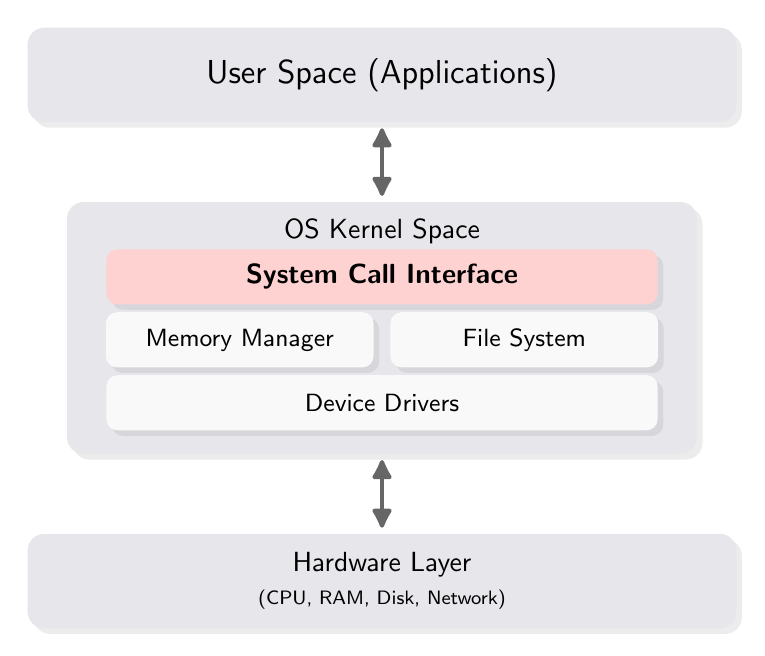
\begin{tikzpicture}[
    node distance=1.0cm,
    font=\sffamily, % 使用無襯線粗體
    % 通用區塊樣式
    block/.style={
        draw=none, 
        rounded corners=6pt, 
        align=center, 
        text=black, % 文字全黑
        drop shadow={opacity=0.15, shadow xshift=2pt, shadow yshift=-2pt}
    },
    % 硬體層樣式 (最底層)
    hardware/.style={
        block, 
        fill=qGrayLight, % 淺灰色背景
        minimum width=9cm, 
        minimum height=1.2cm
    },
    app/.style={
        block, 
        fill=qGrayLight, % 淺灰色背景
        minimum width=9cm, 
        minimum height=1.2cm
    },
    % Kernel 容器樣式 (中間大框)
    kernel_container/.style={
        block, 
        fill=qGrayLight, % 淺藍色背景
        minimum width=8cm, 
        minimum height=3.2cm
    },
    % Kernel 內部小區塊樣式
    subblock/.style={
        block,
        fill=white!95!gray, % 內部用白色突顯
        rounded corners=4pt,
        font=\sffamily\small,
        minimum height=0.7cm
    },
    SP/.style={
        block,
        fill=qPinkLight, % 內部用白色突顯
        rounded corners=4pt,
        font=\sffamily\bfseries,
        minimum height=0.7cm
    },
    % 箭頭樣式 (加粗直徑)
    arrow/.style={
        <->, % 雙向箭頭表示互動
        >={Latex[round, length=3mm, width=3mm]}, 
        draw=black!60, % 箭頭顏色深一點
        line width=1.5pt, 
        shorten >= 2pt, 
        shorten <= 2pt
    }
]

    % --- 1. 建立中心基準線與底層 ---
    % 放置最底層的 Hardware
    \node[hardware] (hw) {Hardware Layer\\ \scriptsize (CPU, RAM, Disk, Network)};

    % --- 2. 建立中層 Kernel (確保置中對齊) ---
    % 放置 Kernel 大容器,位於 Hardware 正上方
    \node[kernel_container, above=1cm of hw] (os) {};
    % 加上 Kernel 標題標籤
    \node[text=black, anchor=north, yshift=-0.1cm] at (os.north) {OS Kernel Space};

    % --- 放置 Kernel 內部元件 (精確定位) ---
    % 放置最上方的 System Call (靠齊容器上方)
    \node[SP, below=0.6cm of os.north, minimum width=7cm] (syscall) {System Call Interface};
    
    % 放置最下方的 Device Drivers (靠齊容器下方)
    \node[subblock, above=0.3cm of os.south, minimum width=7cm] (drivers) {Device Drivers};
    
    % 放置中間的兩個區塊,計算中間點來定位
    \path (syscall.south) -- (drivers.north) coordinate[midway] (midpoint);
    \node[subblock, left=0.1cm of midpoint, anchor=east, minimum width=3.4cm] (mm) {Memory Manager};
    \node[subblock, right=0.1cm of midpoint, anchor=west, minimum width=3.4cm] (fs) {File System};


    % 加上 User Space 標題
    \node[app, text=black, above=1cm of os, font=\sffamily\large] (user) {User Space (Applications)};

    \draw[arrow] (os.north) -- (user.south);

    % Kernel 到 Hardware 的垂直線
    \draw[arrow] (os.south) -- (hw.north);

\end{tikzpicture}

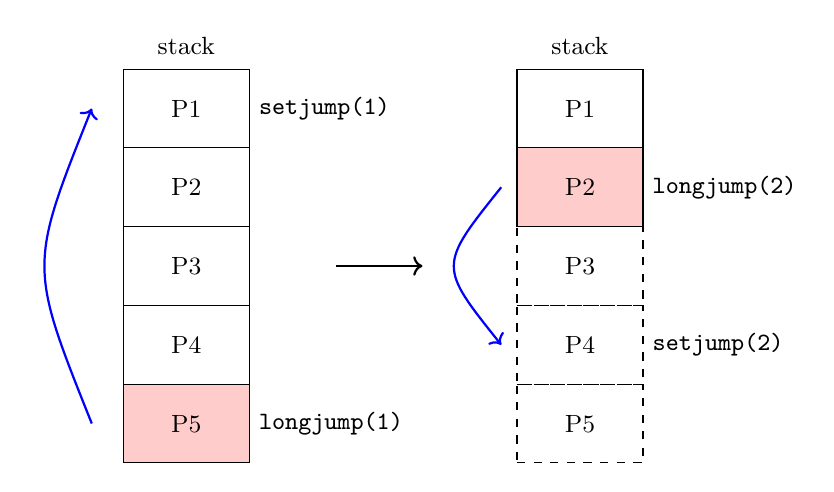
\begin{tikzpicture}[font=\small]

% ==== Left Stack ====
\node at (-2,4.8) {stack};

% Draw stack frames (left)
\foreach \name/\y in {P1/4, P2/3, P3/2, P4/1, P5/0}
    \node[draw, minimum width=1.6cm, minimum height=1cm] (L\name) at (-2,\y) {\name};

% Highlight P5
\node[draw, minimum width=1.6cm, minimum height=1cm, fill=red!20] (LP5) at (-2,0) {P5};

% setjump(1)
\draw (-1.2,4) node[right]{\texttt{setjump(1)}};

% longjump(1)
\draw (-1.2,0) node[right]{\texttt{longjump(1)}};

% Curved arrow left
\draw[->, thick, blue] (-3.2,0) .. controls (-4,2) .. (-3.2,4);


% ===== Arrow to right side =====
\draw[->, thick] (-0.1,2) -- (1.0,2);


% ==== Right Stack ====
\node at (3,4.8) {stack};

% Right stack frames (solid)
\node[draw, minimum width=1.6cm, minimum height=1cm] (RP1) at (3,4) {P1};
\node[draw, minimum width=1.6cm, minimum height=1cm, fill=red!20] (RP2) at (3,3) {P2};

% Dashed frames
\foreach \name/\y in {P3/2, P4/1, P5/0}
    \node[draw, dashed, minimum width=1.6cm, minimum height=1cm] (R\name) at (3,\y) {\name};

% longjump(2)
\draw (3.8,3) node[right]{\texttt{longjump(2)}};

% setjump(2)
\draw (3.8,1) node[right]{\texttt{setjump(2)}};

% Curved arrow right
\draw[->, thick, blue] (2,3) .. controls (1.2,2) .. (2,1);

\end{tikzpicture}

\newpage

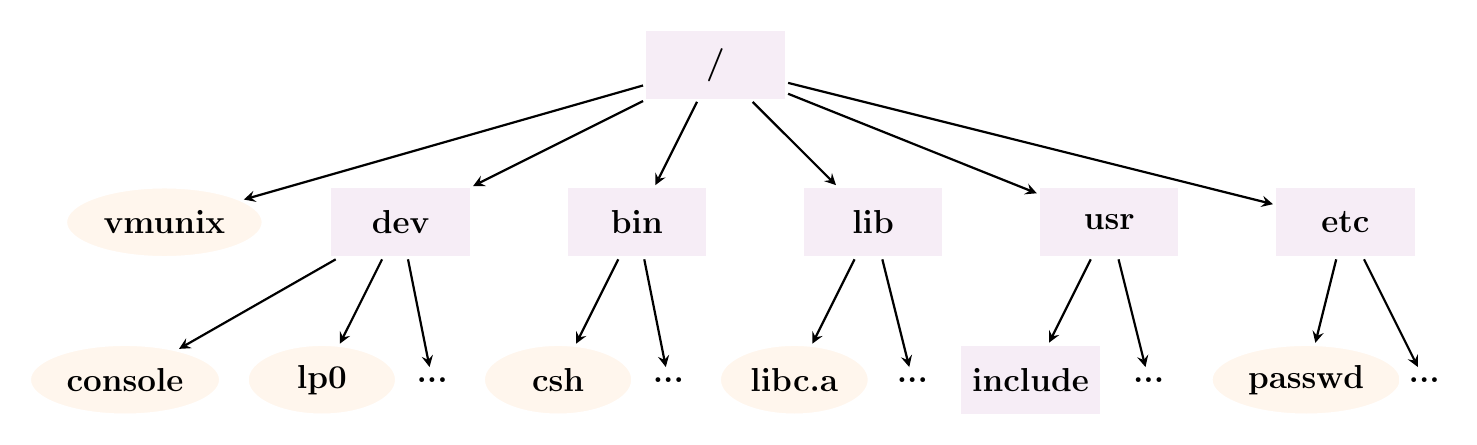
\begin{tikzpicture}[
    x=1cm,y=1cm,
    >=stealth,
    text=white,
    thick,
    box/.style={
        draw=white, very thick,
        rectangle,
        fill=violet!7,
        minimum width=1.8cm,
        minimum height=0.9cm,
        align=center,
        font=\bfseries\large,
        text=black
    },
    oval/.style={
        draw=white, very thick,
        ellipse,
        fill=orange!7,
        minimum width=1.9cm,
        minimum height=0.9cm,
        align=center,
        font=\bfseries\large,
        text=black
    },
    dir/.style={
        draw=none,
        fill=white,
        text=black,
        align=center,
        font=\bfseries\large
    }
]

% ====== 上層節點 ======
\node[box] (root) at (0,0) {/};

\node[box] (dev) at (-4,-2) {dev};
\node[box] (bin) at (-1,-2) {bin};
\node[box] (lib) at ( 2,-2) {lib};
\node[box] (usr) at ( 5,-2) {usr};
\node[box] (etc) at ( 8,-2) {etc};

\node[oval] (vmunix) at (-7,-2) {vmunix};

% root → 第一層
\draw[->] (root) -- (dev);
\draw[->] (root) -- (bin);
\draw[->] (root) -- (lib);
\draw[->] (root) -- (usr);
\draw[->] (root) -- (etc);
\draw[->] (root) -- (vmunix); % 長斜箭頭到 vmunix

% ====== 第二層:dev 下方 ======
\node[oval] (console) at (-7.5,-4) {console};
\node[oval] (lp0)     at (-5.0,-4) {lp0};
\node[dir] (devdot)  at (-3.6,-4) {...};

\draw[->] (dev) -- (console);
\draw[->] (dev) -- (lp0);
\draw[->] (dev) -- (devdot);

% ====== 第二層:bin 下方 ======
\node[oval] (csh)    at (-2.0,-4) {csh};
\node[dir] (bindot) at ( -0.6,-4)  {...};

\draw[->] (bin) -- (csh);
\draw[->] (bin) -- (bindot);

% ====== 第二層:lib 下方 ======
\node[oval] (libca)   at (1.0,-4) {libc.a};
\node[dir] (libdot)  at (2.5,-4) {...};

\draw[->] (lib) -- (libca);
\draw[->] (lib) -- (libdot);

% ====== 第二層:usr 下方 ======
\node[box] (include)  at (4.0,-4) {include};
\node[dir] (usrdot)   at (5.5,-4) {...};

\draw[->] (usr) -- (include);
\draw[->] (usr) -- (usrdot);

% ====== 第二層:etc 下方 ======
\node[oval] (passwd)  at (7.5,-4) {passwd};
\node[dir] (etcdot)  at (9.0,-4) {...};

\draw[->] (etc) -- (passwd);
\draw[->] (etc) -- (etcdot);

\end{tikzpicture}

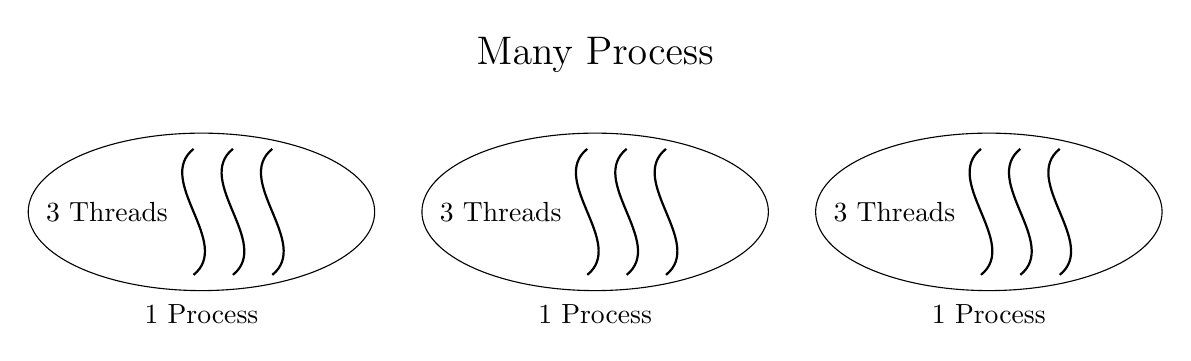
\begin{tikzpicture}[>=stealth, x=1cm, y=1cm]

% Macro: Draw one flattened ellipse with wavy threads
\newcommand{\processthreads}[2]{
\begin{scope}[shift={(#1,0)}]

    % Flattened ellipse
    \draw (0,0) ellipse (2.2cm and 1.0cm);

    % MANY wavy threads inside
    \foreach \x in {-0.1, 0.4, 0.9} {
        \draw[thick]
            (\x,-0.8)
                .. controls (\x+0.5,-0.4) and (\x-0.5,0.4) ..
            (\x,0.8);
    }
    \node at (-1.2, 0) {3 Threads};
    % Label
    \node at (0,-1.3) {#2};

\end{scope}
}

% Draw 3 side-by-side thread groups
\processthreads{-5}{1 Process}
\processthreads{0}{1 Process}
\processthreads{5}{1 Process}

% Optional title
\node at (0,2) {\Large Many Process};

\end{tikzpicture}

\newpage

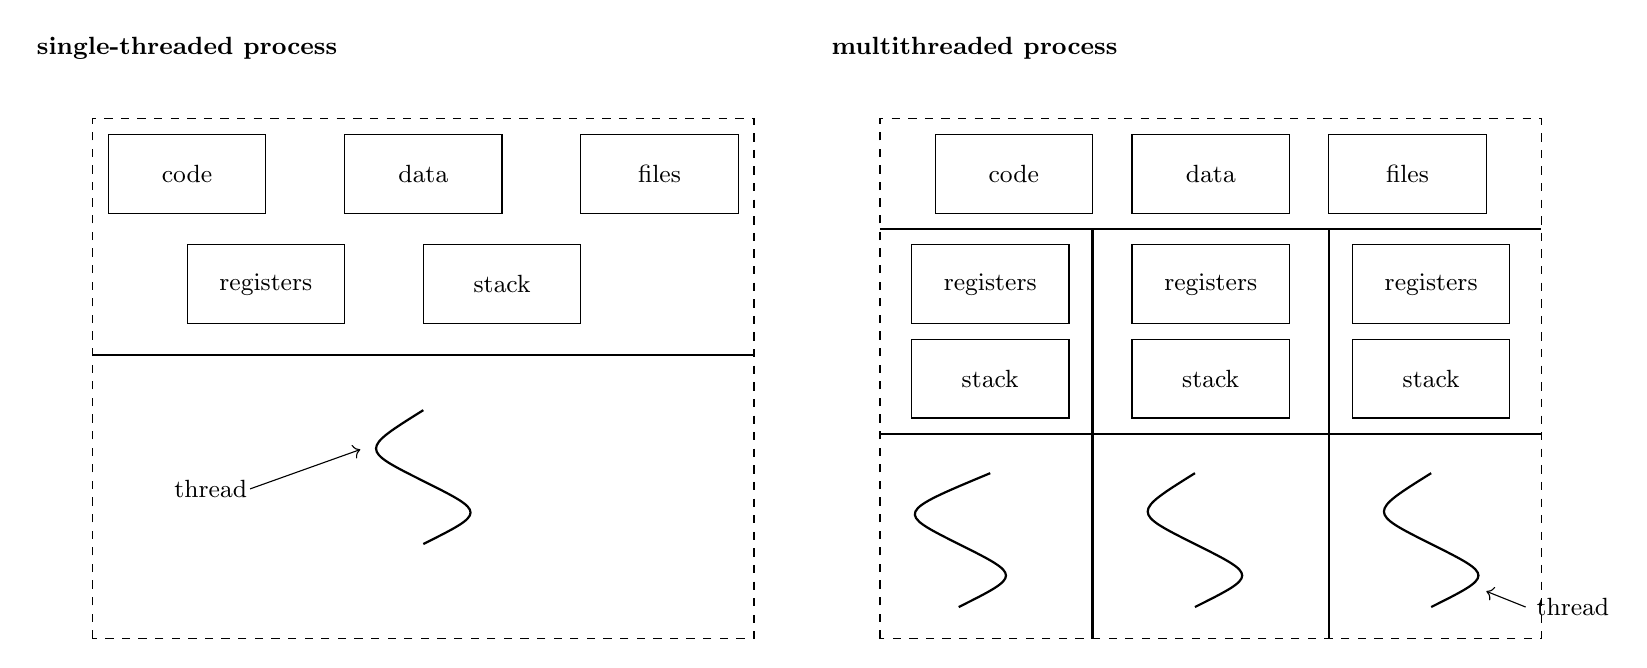
\begin{tikzpicture}[font=\small]

% ===============================================================
% Left: Single-threaded
% ===============================================================

\node at (0,4.2) {\bf single-threaded process};

% dashed outer box
\draw[dashed] (-1.2,-3.3) rectangle (7.2,3.3);

% Top row: code/data/files
\node[draw, minimum width=2cm, minimum height=1cm] (lcode)  at (0,2.6) {code};
\node[draw, minimum width=2cm, minimum height=1cm] (ldata)  at (3,2.6) {data};
\node[draw, minimum width=2cm, minimum height=1cm] (lfiles) at (6,2.6) {files};

% registers + stack row
\node[draw, minimum width=2cm, minimum height=1cm] (lreg)   at (1,1.2) {registers};
\node[draw, minimum width=2cm, minimum height=1cm] (lstack) at (4,1.2) {stack};

% horizontal separator line
\draw[thick] (-1.2,0.3) -- (7.2,0.3);

% Single thread squiggle (3-wave curve)
\draw[thick]
    (3,-0.4) .. controls (2.2,-0.9) .. (3,-1.3)
            .. controls (3.8,-1.7) .. (3,-2.1);

\node at (0.3,-1.4) {thread};
\draw[->] (0.8,-1.4) -- (2.2,-0.9);

% ===============================================================
% Right: Multithreaded
% ===============================================================

\begin{scope}[xshift=10cm]

\node at (0,4.2) {\bf multithreaded process};

% dashed outer box
\draw[dashed] (-1.2,-3.3) rectangle (7.2,3.3);

% Top row: code/data/files
\node[draw, minimum width=2cm, minimum height=1cm] (rcode)  at (0.5,2.6) {code};
\node[draw, minimum width=2cm, minimum height=1cm] (rdata)  at (3,2.6) {data};
\node[draw, minimum width=2cm, minimum height=1cm] (rfiles) at (5.5,2.6) {files};

\draw[thick] (-1.2, 1.9) -- (7.2, 1.9);

% Registers rows
\node[draw, minimum width=2cm, minimum height=1cm] (rreg1) at (0.2,1.2) {registers};
\node[draw, minimum width=2cm, minimum height=1cm] (rreg2) at (3,1.2) {registers};
\node[draw, minimum width=2cm, minimum height=1cm] (rreg3) at (5.8,1.2) {registers};

% Stacks
\node[draw, minimum width=2cm, minimum height=1cm] (rstack1) at (0.2,0) {stack};
\node[draw, minimum width=2cm, minimum height=1cm] (rstack2) at (3,0) {stack};
\node[draw, minimum width=2cm, minimum height=1cm] (rstack3) at (5.8,0) {stack};

% Vertical separators
\draw[thick] (1.5,1.9) -- (1.5,-3.3);
\draw[thick] (4.5,1.9) -- (4.5,-3.3);

% Horizontal separator line
\draw[thick] (-1.2,-0.7) -- (7.2,-0.7);

\def\threadY{-1.2}   % 你要的 thread y 起始位置

% First thread
\draw[thick]
    (0.2,\threadY) .. controls (-1,\threadY-0.5) .. (-0.2,\threadY-0.9)
                    .. controls (0.6,\threadY-1.3) .. (-0.2,\threadY-1.7);

% Second thread
\draw[thick]
    (2.8,\threadY) .. controls (2,\threadY-0.5) .. (2.8,\threadY-0.9)
                    .. controls (3.6,\threadY-1.3) .. (2.8,\threadY-1.7);

% Third thread
\draw[thick]
    (5.8,\threadY) .. controls (5,\threadY-0.5) .. (5.8,\threadY-0.9)
                    .. controls (6.6,\threadY-1.3) .. (5.8,\threadY-1.7);


% Thread arrow
\node at (7.6,\threadY-1.7) {thread};
\draw[->] (7,\threadY-1.7) -- (6.5,\threadY-1.5);

\end{scope}

\end{tikzpicture}

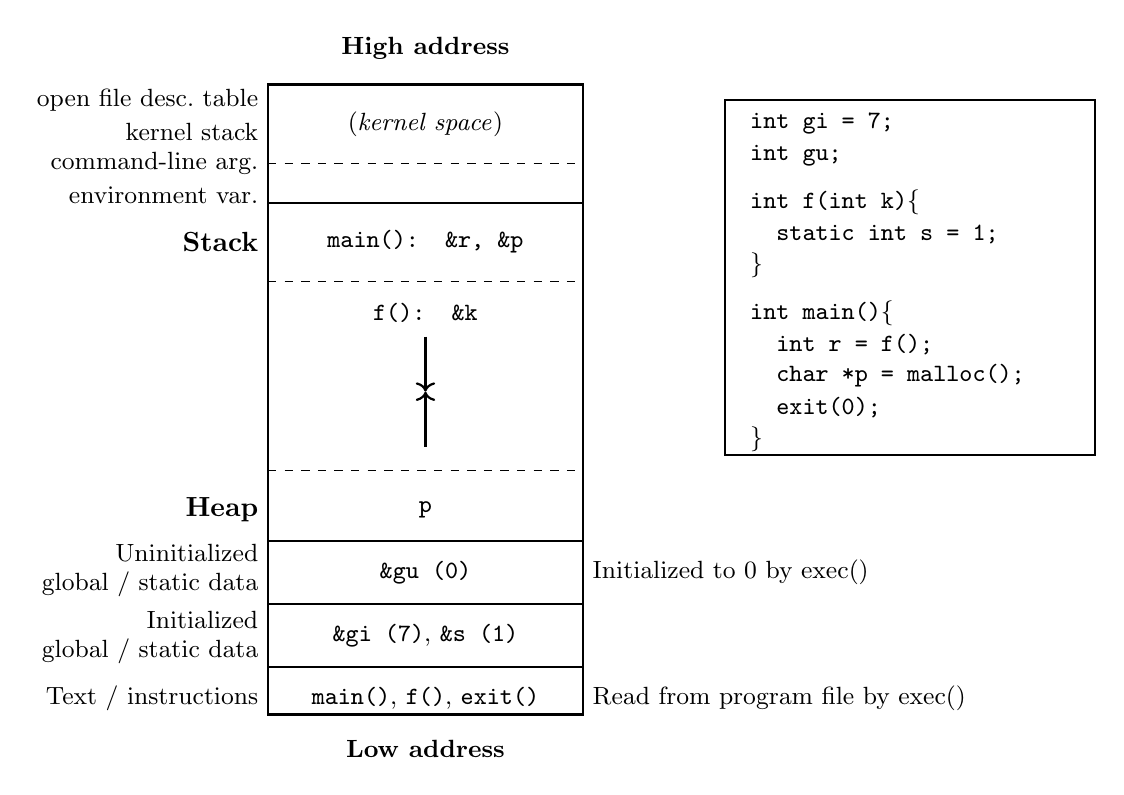
\begin{tikzpicture}[font=\small]

% ========================
% LEFT LABELS (aligned right to x=0)
% ========================

% Left labels baseline positions (re-aligned)
\node[anchor=east] at (0,3.8) {open file desc.\ table};
\node[anchor=east] at (0,3.4) {kernel stack};
\node[anchor=east] at (0,3.0) {command-line arg.};
\node[anchor=east] at (0,2.6) {environment var.};

\node[anchor=east,font=\bfseries] at (0,2.0) {Stack};

\node[anchor=east,font=\bfseries] at (0,-1.4) {Heap};

\node[anchor=east] at (0,-1.95) {Uninitialized};
\node[anchor=east] at (0,-2.35) {global / static data};

\node[anchor=east] at (0,-2.8) {Initialized};
\node[anchor=east] at (0,-3.2) {global / static data};

\node[anchor=east] at (0,-3.8) {Text / instructions};


% ========================
% MAIN MEMORY BLOCK
% ========================

\draw[thick] (0,4) rectangle (4,-4);

% kernel space
\node at (2,3.5) {(\textit{kernel space})};

\draw[dashed] (0,3.0) -- (4,3.0);

% main(): &r &p
\node at (2,2) {{\texttt{main(): \&r, \&p}}};
\draw[thick] (0,2.5) -- (4,2.5);

% f(): &k
\draw[dashed] (0,1.5) -- (4,1.5);
\node at (2,1.1) {{\texttt{f(): \&k}}};

% stack downward arrow
\draw[->,thick] (2,0.8) -- (2,0.1);
\draw[<-,thick] (2,0.1) -- (2,-0.6);

% heap p
\draw[dashed] (0,-0.9) -- (4,-0.9);
\node at (2,-1.4) {\texttt{p}};

\draw[thick] (0,-1.8) -- (4,-1.8);

% uninitialized global/static
\node at (2,-2.2) {\texttt{\&gu (0)}};
\draw[thick] (0,-2.6) -- (4,-2.6);

% initialized global/static
\node at (2,-3.0) {\texttt{\&gi (7)}, \texttt{\&s (1)}};
\draw[thick] (0,-3.4) -- (4,-3.4);

% text / instructions
\node at (2,-3.8) {\texttt{main()}, \texttt{f()}, \texttt{exit()}};

% Address labels
\node[anchor=south] at (2,4.2) {\bf High address};
\node[anchor=north] at (2,-4.2) {\bf Low address};


% ========================
% RIGHT CODE BLOCK (with border)
% ========================

\begin{scope}[xshift=7.5cm]

\draw[thick] (-1.7,3.8) rectangle (3,-0.7);  % code box frame

\node[anchor=west] at (-1.5,3.5) {\texttt{int gi = 7;}};
\node[anchor=west] at (-1.5,3.1) {\texttt{int gu;}};

\node[anchor=west] at (-1.5,2.5) {\texttt{int f(int k)\{}};
\node[anchor=west] at (-1.5,2.1) {\texttt{\ \ static int s = 1;}};
\node[anchor=west] at (-1.5,1.7) {\texttt{\}}};

\node[anchor=west] at (-1.5,1.1) {\texttt{int main()\{}};
\node[anchor=west] at (-1.5,0.7) {\texttt{\ \ int r = f();}};
\node[anchor=west] at (-1.5,0.3) {\texttt{\ \ char *p = malloc();}};
\node[anchor=west] at (-1.5,-0.1) {\texttt{\ \ exit(0);}};
\node[anchor=west] at (-1.5,-0.5) {\texttt{\}}};

% right-side comments
\node[anchor=west] at (-3.5,-2.2) {Initialized to 0 by exec()};
\node[anchor=west] at (-3.5,-3.8) {Read from program file by exec()};

\end{scope}

\end{tikzpicture}

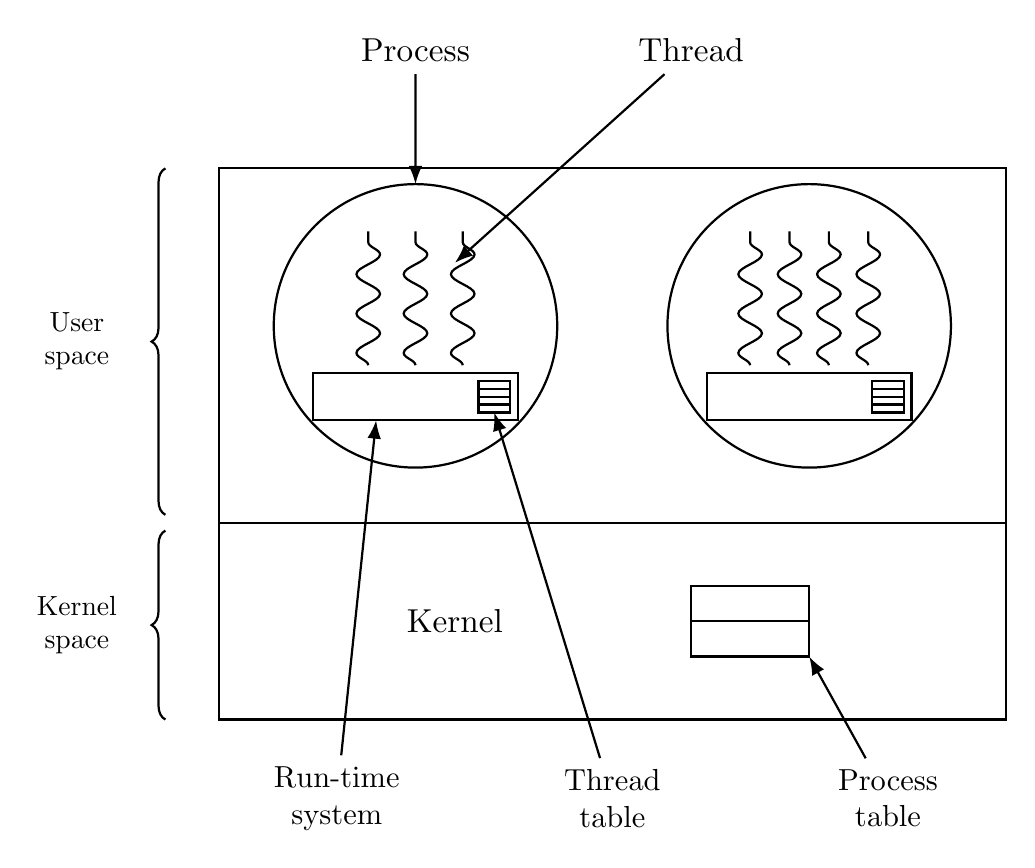
\begin{tikzpicture}[
    >=Latex, % 使用漂亮的箭頭
    thick,
    box/.style={draw, thick, fill=white},
    thread/.style={decorate, decoration={snake, amplitude=1.5mm, segment length=5mm, post length=0mm}, thick}
]

    % --- 1. 定義坐標與區域 ---
    % 畫外框 (Main Box)
    \draw[thick] (0,0) rectangle (10, 7);
    
    % 畫分隔線 (Separation Line)
    \draw[thick] (0, 2.5) -- (10, 2.5);
    
    % --- 2. 文字標籤 (左側大括號) ---
    % User space brace
    \draw [decorate, decoration={brace, amplitude=5pt, raise=5pt}]
    (-0.5, 2.6) -- (-0.5, 7) node [midway, xshift=-1.3cm, align=center] {User\\space};
    
    % Kernel space brace
    \draw [decorate, decoration={brace, amplitude=5pt, raise=5pt}]
    (-0.5, 0) -- (-0.5, 2.4) node [midway, xshift=-1.3cm, align=center] {Kernel\\space};
    % Kernel 文字
    \node at (3, 1.25) [scale=1.2] {Kernel};


    % --- 3. 繪製 Process (圓圈) ---
    
    % Process 1 (左邊)
    \draw[thick] (2.5, 5) circle (1.8cm);
    
    % Process 2 (右邊)
    \draw[thick] (7.5, 5) circle (1.8cm);

    % --- 4. 繪製 Process 內部的 Run-time system 和 Threads ---
    
    % 定義一個 macro 來畫內部的東西,方便重複
    \newcommand{\drawInternals}[2]{
        % 參數 #1: 中心 x 座標
        % 參數 #2: 執行緒數量 (3 或 4)
        
        % Run-time system 矩形框
        \draw[thick, fill=white] (#1-1.3, 3.8) rectangle (#1+1.3, 4.4);
        
        % Thread table (Run-time system 裡面的小格子)
        \draw[thick] (#1+0.8, 3.9) rectangle (#1+1.2, 4.3);
        \draw (#1+0.8, 4.1) -- (#1+1.2, 4.1); % 中間橫線
        \draw (#1+0.8, 4.0) -- (#1+1.2, 4.0); 
        \draw (#1+0.8, 4.2) -- (#1+1.2, 4.2);

        % Threads (波浪線)
        \ifnum#2=3
            \draw[thread] (#1-0.6, 4.5) -- (#1-0.6, 6.2);
            \draw[thread] (#1, 4.5) -- (#1, 6.2);
            \draw[thread] (#1+0.6, 4.5) -- (#1+0.6, 6.2);
        \else
            \draw[thread] (#1-0.75, 4.5) -- (#1-0.75, 6.2);
            \draw[thread] (#1-0.25, 4.5) -- (#1-0.25, 6.2);
            \draw[thread] (#1+0.25, 4.5) -- (#1+0.25, 6.2);
            \draw[thread] (#1+0.75, 4.5) -- (#1+0.75, 6.2);
        \fi
    }

    % 畫左邊 Process 的內容
    \drawInternals{2.5}{3}
    
    % 畫右邊 Process 的內容
    \drawInternals{7.5}{4}


    % --- 5. 繪製 Kernel 中的 Process Table ---
    \draw[thick] (6, 0.8) rectangle (7.5, 1.7);
    \draw[thick] (6, 1.25) -- (7.5, 1.25); % 中間橫線


    % --- 6. 外部標註與箭頭 (Arrows & Labels) ---
    
    % Process Label
    \node (lbl_proc) at (2.5, 8.5) [scale=1.2] {Process};
    \draw[->, thick] (lbl_proc) -- (2.5, 6.8); % 指向圓圈頂部

    % Thread Label
    \node (lbl_thread) at (6, 8.5) [scale=1.2] {Thread};
    \draw[->, thick] (lbl_thread) -- (3, 5.8); % 指向中間的波浪線

    % Run-time system Label
    \node (lbl_runtime) at (1.5, -1) [scale=1.1, align=center] {Run-time\\system};
    \draw[->, thick] (lbl_runtime) -- (2, 3.8); % 指向矩形框

    % Thread table Label
    \node (lbl_ttable) at (5, -1) [scale=1.1, align=center] {Thread\\table};
    \draw[->, thick] (lbl_ttable) -- (3.5, 3.9); % 指向裡面的小格子

    % Process table Label
    \node (lbl_ptable) at (8.5, -1) [scale=1.1, align=center] {Process\\table};
    \draw[->, thick] (lbl_ptable) -- (7.5, 0.8); % 指向 Kernel 表格

\end{tikzpicture}


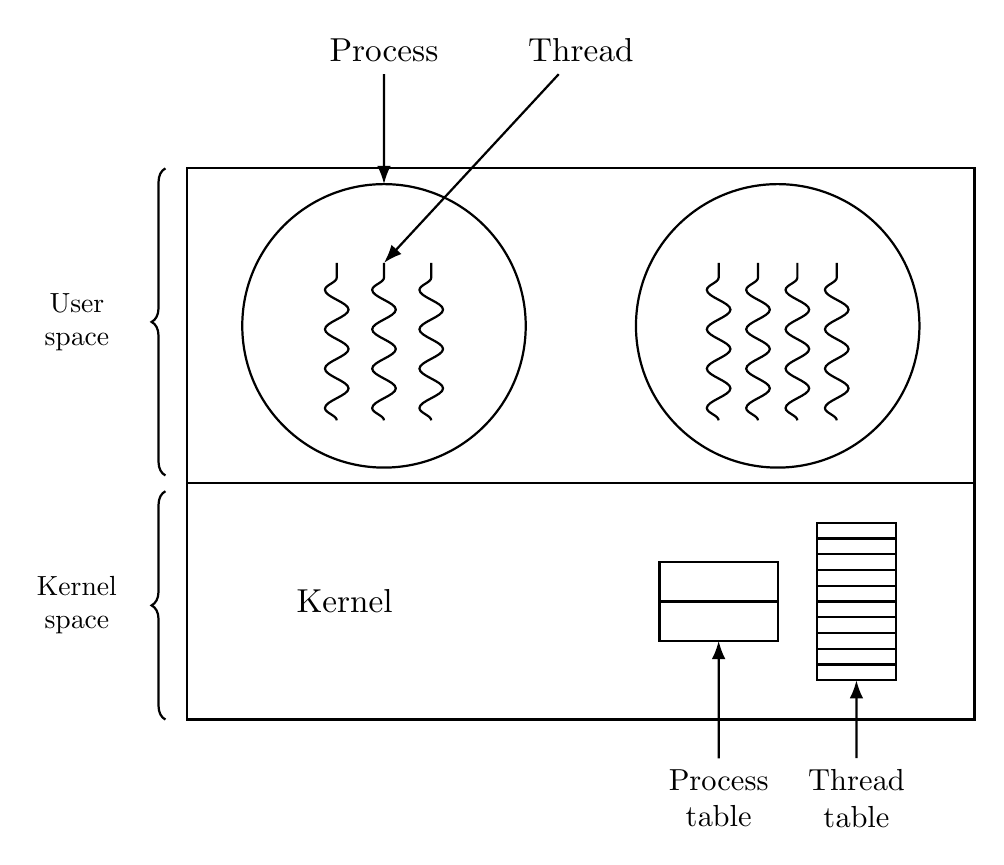
\begin{tikzpicture}[
    >=Latex, % 使用漂亮的箭頭
    thick,
    box/.style={draw, thick, fill=white},
    thread/.style={decorate, decoration={snake, amplitude=1.5mm, segment length=5mm, post length=0mm}, thick}
]

    % --- 1. 定義坐標與區域 ---
    % 畫外框 (Main Box)
    \draw[thick] (0,0) rectangle (10, 7);
    
    % 畫分隔線 (Separation Line) - 這次線比較低一點,讓 Kernel 空間變大
    \draw[thick] (0, 3) -- (10, 3);
    
    % --- 2. 文字標籤 (左側大括號) ---
    % User space brace
    \draw [decorate, decoration={brace, amplitude=5pt, raise=5pt}]
    (-0.1, 3.1) -- (-0.1, 7) node [midway, xshift=-1.3cm, align=center] {User\\space};
    
    % Kernel space brace
    \draw [decorate, decoration={brace, amplitude=5pt, raise=5pt}]
    (-0.1, 0) -- (-0.1, 2.9) node [midway, xshift=-1.3cm, align=center] {Kernel\\space};

    % Kernel 文字
    \node at (2, 1.5) [scale=1.2] {Kernel};


    % --- 3. 繪製 Process (圓圈) ---
    
    % Process 1 (左邊)
    \draw[thick] (2.5, 5) circle (1.8cm);
    
    % Process 2 (右邊)
    \draw[thick] (7.5, 5) circle (1.8cm);

    % --- 4. 繪製 Process 內部的 Threads (波浪線) ---
    % 這次只需要畫波浪線,沒有內部的矩形框了
    
    % 定義一個 macro 來畫波浪線
    \newcommand{\drawThreads}[2]{
        % 參數 #1: 中心 x 座標
        % 參數 #2: 執行緒數量 (3 或 4)
        \ifnum#2=3
            \draw[thread] (#1-0.6, 3.8) -- (#1-0.6, 5.8);
            \draw[thread] (#1, 3.8) -- (#1, 5.8);
            \draw[thread] (#1+0.6, 3.8) -- (#1+0.6, 5.8);
        \else
            \draw[thread] (#1-0.75, 3.8) -- (#1-0.75, 5.8);
            \draw[thread] (#1-0.25, 3.8) -- (#1-0.25, 5.8);
            \draw[thread] (#1+0.25, 3.8) -- (#1+0.25, 5.8);
            \draw[thread] (#1+0.75, 3.8) -- (#1+0.75, 5.8);
        \fi
    }

    % 畫左邊 Process 的 Threads
    \drawThreads{2.5}{3}
    
    % 畫右邊 Process 的 Threads
    \drawThreads{7.5}{4}


    % --- 5. 繪製 Kernel 中的 Tables ---
    
    % Process Table (左邊那個)
    \draw[thick] (6, 1) rectangle (7.5, 2);
    \draw[thick] (6, 1.5) -- (7.5, 1.5); % 中間橫線

    % Thread Table (右邊那個,這次很多格)
    \draw[thick] (8, 0.5) rectangle (9, 2.5);
    \foreach \y in {0.7, 0.9, 1.1, 1.3, 1.5, 1.7, 1.9, 2.1, 2.3} {
        \draw (8, \y) -- (9, \y);
    }


    % --- 6. 外部標註與箭頭 (Arrows & Labels) ---
    
    % Process Label
    \node (lbl_proc) at (2.5, 8.5) [scale=1.2] {Process};
    \draw[->, thick] (lbl_proc) -- (2.5, 6.8); % 指向圓圈頂部

    % Thread Label
    \node (lbl_thread) at (5, 8.5) [scale=1.2] {Thread};
    \draw[->, thick] (lbl_thread) -- (2.5, 5.8); % 指向左邊 Process 的中間波浪線

    % Process table Label
    \node (lbl_ptable) at (6.75, -1) [scale=1.1, align=center] {Process\\table};
    \draw[->, thick] (lbl_ptable) -- (6.75, 1); % 指向左邊的表格

    % Thread table Label
    \node (lbl_ttable) at (8.5, -1) [scale=1.1, align=center] {Thread\\table};
    \draw[->, thick] (lbl_ttable) -- (8.5, 0.5); % 指向右邊的表格

\end{tikzpicture}

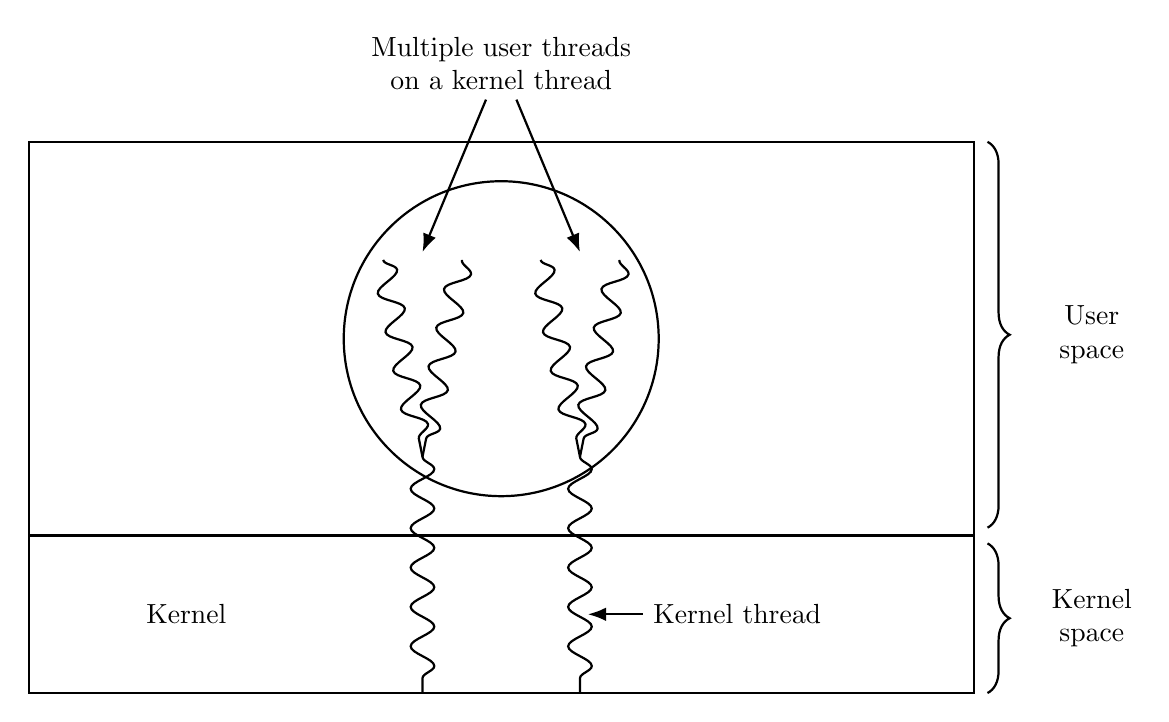
\begin{tikzpicture}[
    >=Latex,
    thick,
    % 調整波浪樣式:segment length 越大,波浪越平緩(數量越少)
    mythread/.style={decorate, decoration={snake, amplitude=1.5mm, segment length=5mm}, thick}
]

% --- 1. 外框與分隔線 ---
\draw (0,0) rectangle (12, 7);
\draw (0, 2) -- (12, 2); % 分隔線
\node at (2, 1) {Kernel};

% --- 2. Process (圓圈) ---
\coordinate (center) at (6, 4.5);
\draw (center) circle (2);

% --- 3. 繪製執行緒 (Threads) ---

% --- 左邊的群組 (Left Group) ---
\coordinate (merge_left) at (5, 3); % 合併點

% User threads (兩條合併)
\draw[mythread] (4.5, 5.5) -- (merge_left);
\draw[mythread] (5.5, 5.5) -- (merge_left);

% Kernel thread (向下延伸)
\draw[mythread] (merge_left) -- (5, 0);


% --- 右邊的群組 (Right Group) ---
\coordinate (merge_right) at (7, 3); % 合併點

% User threads (兩條合併)
\draw[mythread] (6.5, 5.5) -- (merge_right);
\draw[mythread] (7.5, 5.5) -- (merge_right);

% Kernel thread (向下延伸)
\draw[mythread] (merge_right) -- (7, 0);


% --- 4. 標示與箭頭 ---

% 上方標籤
\node[align=center] (top_label) at (6, 8) {Multiple user threads\\on a kernel thread};
\draw[->, thick] (top_label) -- (5, 5.6); % 指向左邊群組
\draw[->, thick] (top_label) -- (7, 5.6); % 指向右邊群組

% 下方標籤 (Kernel thread)
\node[anchor=west] (k_label) at (7.8, 1) {Kernel thread};
\draw[->, thick] (k_label) -- (7.1, 1); % 指向右邊的 Kernel thread 線條

% --- 5. 右側大括號 ---
% User space
\draw[decorate, decoration={brace, mirror, amplitude=8pt, raise=5pt}] 
    (12, 2.1) -- (12, 7) node[midway, xshift=1.5cm, align=center] {User\\space};

% Kernel space
\draw[decorate, decoration={brace, mirror, amplitude=8pt, raise=5pt}] 
    (12, 0) -- (12, 1.9) node[midway, xshift=1.5cm, align=center] {Kernel\\space};

\end{tikzpicture}

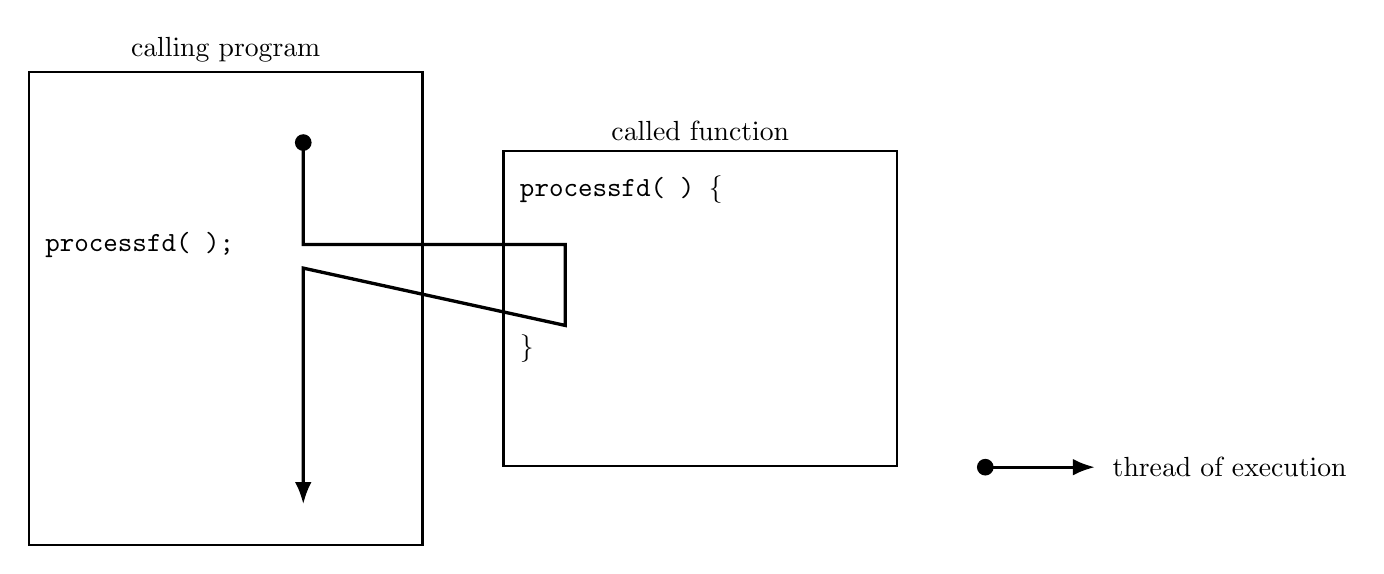
\begin{tikzpicture}[
    % 全域樣式設定
    code text/.style={font=\ttfamily, anchor=west}, % 程式碼文字使用等寬字體
    box/.style={draw, thick, rectangle, minimum width=5cm, minimum height=6cm}, % 方框樣式
    % 定義執行緒路徑的線條樣式:非常粗,起點有圓點,終點有箭頭
    thread path/.style={very thick, {Circle[length=6pt]}-{Latex[length=8pt, width=6pt]}}
]

    % --- 1. 繪製左側的方框 (calling program) ---
    \node[box] (caller) at (0,0) {};
    % 標題
    \node[above] at (caller.north) {calling program};
    % 內部的程式碼文字 (使用相對座標定位)
    \node[code text] at ($(caller.north west) + (0.1, -2.2)$) {processfd( );};


    % --- 2. 繪製右側的方框 (called function) ---
    % 位置在左側方框的右邊,稍微往上偏移以符合原圖
    \node[box, right=1cm of caller, minimum height=4cm] (callee) {};
    % 標題
    \node[above] at (callee.north) {called function};
    % 內部的程式碼文字
    \node[code text] at ($(callee.north west) + (0.1, -0.5)$) {processfd( ) \{};
    \node[code text] at ($(callee.south west) + (0.1, 1.5)$) {\}};


    % --- 3. 繪製執行緒路徑 (Thread of execution path) ---
    % 定義路徑的關鍵轉折點座標
    % 起點圓點
    \coordinate (p_start) at ($(caller.north west) + (3.5, -0.8)$);
    % 第一個轉折 (向下到呼叫點)
    \coordinate (p_call) at ($(caller.north west) + (3.5, -2.2)$);
    % 進入函數點
    \coordinate (p_enter) at ($(callee.north west) + (0.8, -1.2)$);
    % 函數內部結束點
    \coordinate (p_exit) at ($(callee.south west) + (0.8, 1.8)$);
    % 返回轉折點
    \coordinate (p_return) at ($(caller.north west) + (3.5, -2.5)$);
    % 最終結束點 (箭頭處)
    \coordinate (p_end) at ($(caller.north west) + (3.5, -5.5)$);

    % 繪製連續的路徑線條
    \draw[thread path] (p_start) -- (p_call) -- (p_enter) -- (p_exit) -- (p_return) -- (p_end);


    % --- 4. 繪製圖例 (Legend) ---
    % 定義圖例的位置在右側方框的右下方
    \begin{scope}[shift={($(callee.south east) + (1, 0)$)}]
        % 繪製範例線條
        \draw[thread path] (0,0) -- (1.5, 0);
        % 繪製文字說明
        \node[anchor=west] at (1.6, 0) {thread of execution};
    \end{scope}

\end{tikzpicture}

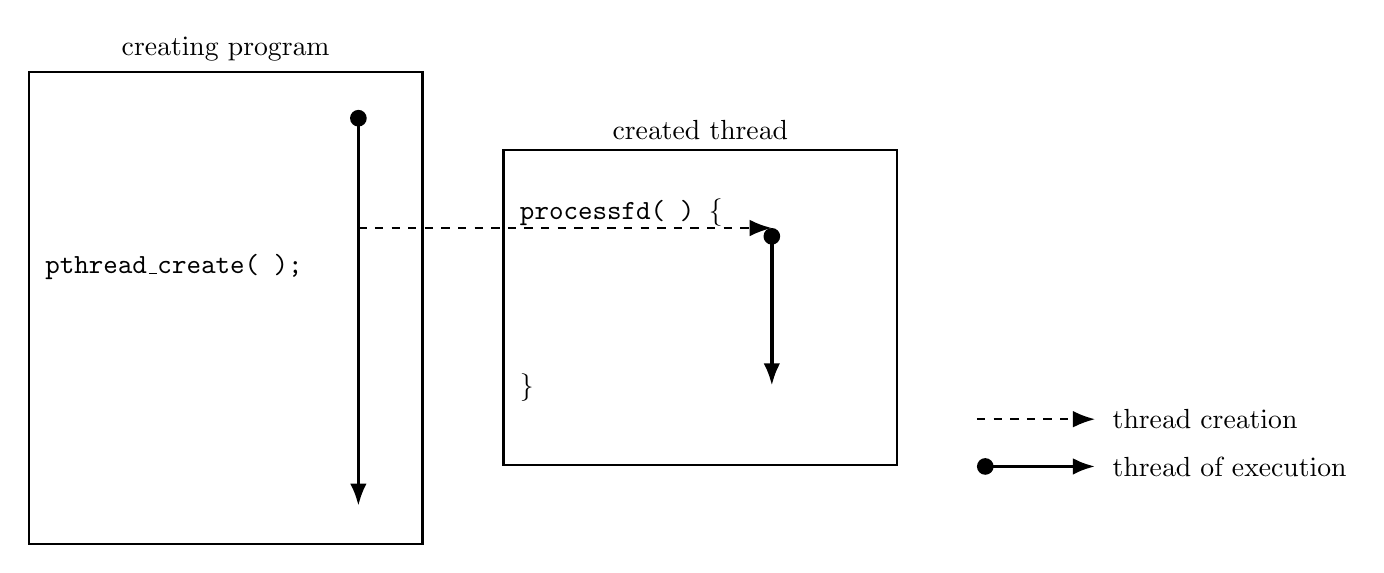
\begin{tikzpicture}[
    % --- 全域樣式設定 (保留你的設定) ---
    code text/.style={font=\ttfamily, anchor=west}, 
    box/.style={draw, thick, rectangle, minimum width=5cm, minimum height=6cm}, 
    % 實線路徑 (Thread of execution)
    thread path/.style={very thick, {Circle[length=6pt]}-{Latex[length=8pt, width=6pt]}},
    % 虛線路徑 (Thread creation)
    create path/.style={thick, dashed, -{Latex[length=8pt, width=6pt]}}
]

    % --- 1. 繪製左側的方框 (creating program) ---
    \node[box] (creator) at (0,0) {};
    \node[above] at (creator.north) {creating program};
    \node[code text] (p_create) at ($(creator.north west) + (0.1, -2.5)$) {pthread\_create( );};


    % --- 2. 繪製右側的方框 (created thread) ---
    \node[box, right=1cm of creator, minimum height=4cm] (created) {};
    \node[above] at (created.north) {created thread};
    % 給它一個名稱 (p_func) 方便定位X軸
    \node[code text] (p_func) at ($(created.north west) + (0.1, -0.8)$) {processfd( ) \{};
    \node[code text] at ($(created.south west) + (0.1, 1.0)$) {\}};


    % --- 3. 繪製路徑 (Paths) ---
    
    % A. 定義關鍵座標 (修改重點在此)
    
    % [1. 定義左側主執行緒的 X 軸位置參考]
    % 設在方框左上角往右 4.2cm 處
    \coordinate (t1_x_ref) at ($(creator.north west) + (4.2, 0)$);

    % [2. 定義分岔點 (Fork Point)]
    % X 軸取自參考點 t1_x_ref,Y 軸取自文字 p_create 的中心
    % 這保證了點在主執行緒線上,且高度對齊文字
    \coordinate (fork_point) at (t1_x_ref |- p_create);

    % [3. 定義左側主執行緒的起點與終點]
    % 利用參考點的 X,設定上下高度
    \coordinate (t1_top) at (t1_x_ref |- creator.north west); % 稍微調整高度對齊方框頂
    \coordinate (t1_bottom) at ($(t1_x_ref |- creator.south west) + (0, 0.5)$); % 稍微調整高度在方框底上面

    % [4. 定義右側新執行緒的起點 (關鍵修改!)]
    % 我們先找一個右側的 X 軸參考位置 (在 processfd 文字右邊 0.5cm)
    \coordinate (t2_x_ref) at ($(p_func.east) + (0.5, 0)$);
    % **關鍵步驟**:新執行緒的起點 (t2_start)
    % X 軸取自 t2_x_ref,**Y 軸強制取自 fork_point**
    % 這樣保證了 t2_start 和 fork_point 在同一高度,連線就會是水平的
    \coordinate (t2_start) at (t2_x_ref |- fork_point);

    % [5. 定義右側新執行緒的終點]
    % 從起點垂直往下 2.5cm
    \coordinate (t2_end) at ($(t2_start) + (0, -2.5)$);
    

    % B. 繪製線條
    
    % 畫左邊垂直線 (主程式)
    % 這裡起點稍微往下移一點點,避開方框邊緣,視覺更好看
    \draw[thread path] ($(t1_top)+(0,-0.5)$) -- (t1_bottom);
    
    % 畫右邊垂直線 (新執行緒)
    \draw[thread path] ($(t2_start) + (0, 0.5)$) -- ($(t2_end) + (0, 1)$);
    
    % 畫中間虛線 (建立動作)
    % 因為 fork_point 和 t2_start 高度一致,這條線現在是完美水平的
    \draw[create path] ($(fork_point) + (0, 0.5)$) -- ($(t2_start) + (0, 0.5)$);


    % --- 4. 繪製圖例 (Legend) ---
    \begin{scope}[shift={($(created.south east) + (1, 0)$)}]
        \draw[create path] (0, 0.6) -- (1.5, 0.6);
        \node[anchor=west] at (1.6, 0.6) {thread creation};
        
        \draw[thread path] (0, 0) -- (1.5, 0);
        \node[anchor=west] at (1.6, 0) {thread of execution};
    \end{scope}

\end{tikzpicture}

\tikzset{
    % 1. "main thread" 和 "spawned thread" 的方塊樣式 (強調:粗框)
    threadbox/.style={
        draw=black,            
        line width=2pt,        
        fill=white,            
        text=black,            
        font=\Large,
        align=center,
        minimum width=3.5cm,
        minimum height=1.8cm
    },
    % 2. 函數調用 (pthread_...) 的方塊樣式 (一般:細框 + 等寬字體)
    funcbox/.style={
        draw=black,            
        line width=1pt,        
        fill=white,            
        text=black,            
        font=\ttfamily\bfseries\large,
        inner sep=8pt
    },
    % 3. 箭頭樣式
    arrow/.style={
        ->,
        >={Latex[scale=1.5, length=3mm, width=4mm]},
        line width=2pt,
        draw=black
    },
    % 4. "DO WORK" 文字標籤樣式
    doworkLabel/.style={
        text=black,
        fill=white,
        font=\Large,   
    }
}

\begin{tikzpicture}[
    node distance=2cm and 3cm
]

    % --- 放置節點 ---

    % 第一列:Main Thread 和建立流程
    \node[threadbox] (main) {main\\thread};
    
    \node[funcbox, right=of main] (create) {pthread\_create()};
    \node[funcbox, right=4cm of create] (join) {pthread\_join()};
    
    % 隱形終點
    \coordinate[right=2cm of join] (end);

    % 第二列:產生的執行緒
    \node[threadbox, below=of create] (spawn1) {spawned\\thread};
    \node[threadbox, below=0.5cm of spawn1] (spawn2) {spawned\\thread};

    % 第三部分:Exit 節點
    \node[funcbox] (exit) at (join |- spawn1) {pthread\_exit()};


    % --- 繪製連接箭頭 ---

    % 1. 上方水平流程
    \draw[arrow] (main) -- (create);
    \draw[arrow] (create) -- (join);
    \draw[arrow] (join) -- (end);

    % 2. 向下建立執行緒的流程
    \draw[arrow] (create) -- (spawn1);

    % 3. 工作和退出流程 (DO WORK -> exit)
    \draw[arrow] ($(spawn1.east)!0.5!(spawn2.east)$) -- 
        node[doworkLabel, midway] {DO WORK} 
        (exit.west);

    % 4. 向上會合流程 (exit -> join)
    \draw[arrow] (exit) -- (join);

\end{tikzpicture}


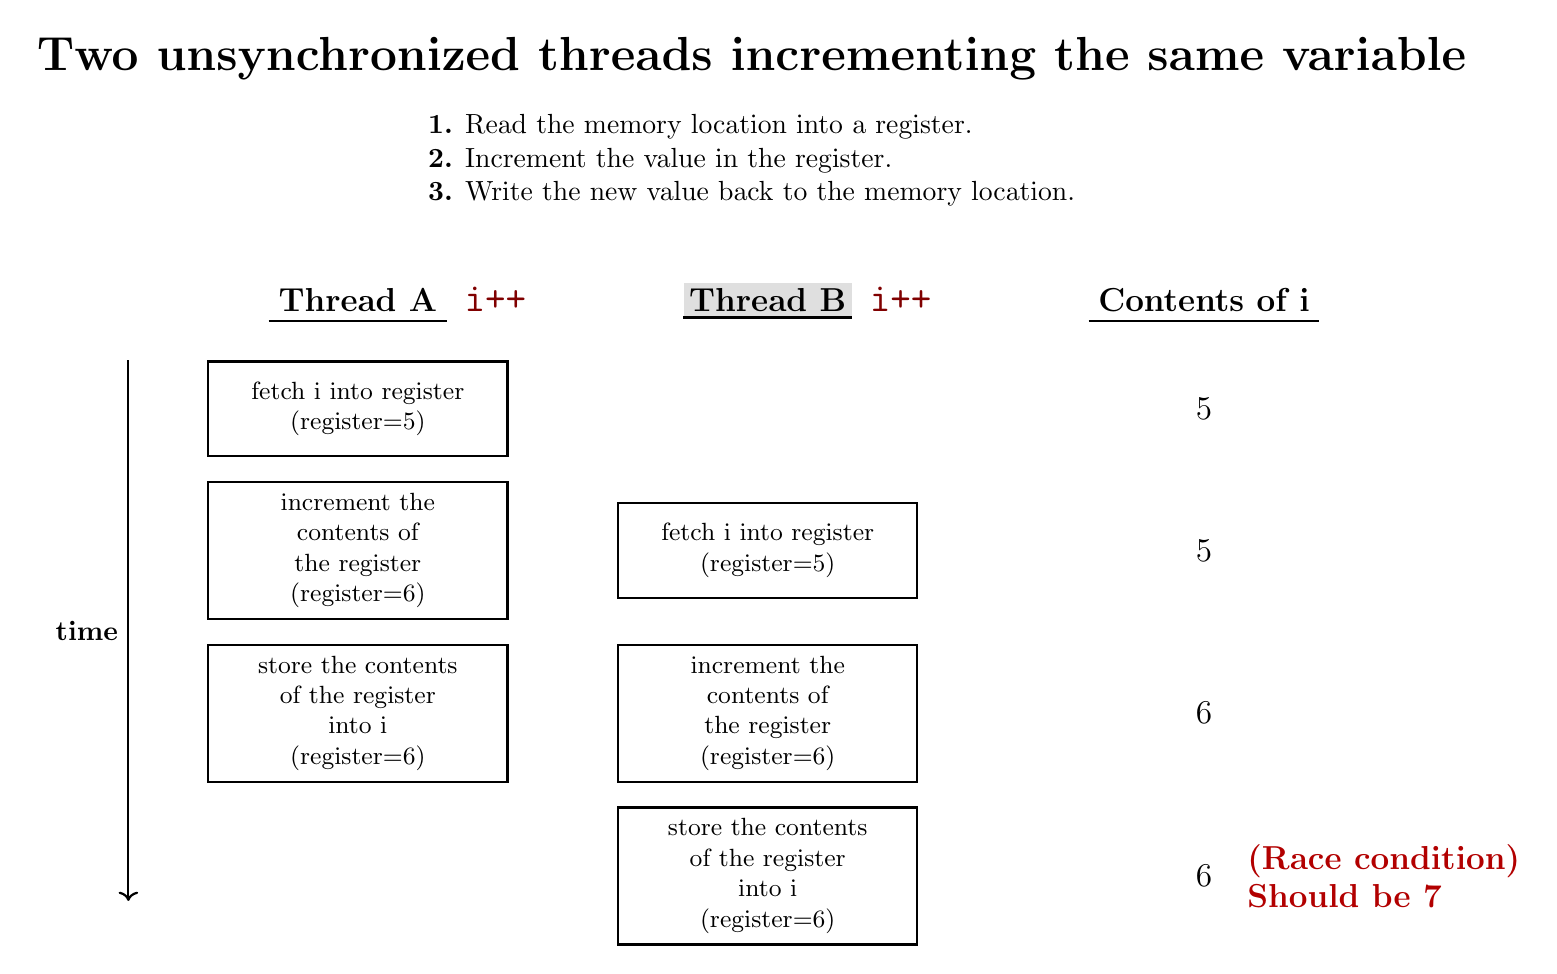
\begin{tikzpicture}[
    font=\sffamily,
    % 定義方框樣式
    opbox/.style={
        draw=black,
        thick,
        fill=white,
        align=center,
        font=\small,
        inner sep=4pt,
        minimum width=3.8cm,
        minimum height=1.2cm
    },
    % 定義數值文字樣式
    valtext/.style={
        font=\large,
        align=center
    },
    % 定義標題樣式
    header/.style={
        font=\bfseries\large,
        align=center
    }
]

    % --- 1. 頂部文字區塊 ---
    \node[font=\bfseries\LARGE, align=center] (title) at (0,0) {Two unsynchronized threads incrementing the same variable};
    
    \node[below=0.2cm of title, align=left, font=\normalsize] (list) {
        \textbf{1.} Read the memory location into a register.\\
        \textbf{2.} Increment the value in the register.\\
        \textbf{3.} Write the new value back to the memory location.
    };

    % --- 2. 表頭 (Headers) ---
    % Thread A
    \node[header, below=0.8cm of list, xshift=-5cm] (hA) {Thread A};
    \draw[thick] (hA.south west) -- (hA.south east);
    \node[right=0.1cm of hA, font=\bfseries\Large\color{red!50!black}] {\texttt{i++}};

    % Thread B (灰色背景)
    \node[header, right=3cm of hA, fill=lightgray!50, inner sep=2pt] (hB) {Thread B};
    \draw[thick] (hB.south west) -- (hB.south east);
    \node[right=0.1cm of hB, font=\bfseries\Large\color{red!50!black}] {\texttt{i++}};

    % Contents of i
    \node[header, right=3cm of hB] (hC) {Contents of i};
    \draw[thick] (hC.south west) -- (hC.south east);


    % --- 3. 流程圖內容 (Rows) ---

    % Row 1: A Fetch, i=5
    \node[opbox, below=0.5cm of hA] (a1) {fetch i into register\\(register=5)};
    \node[valtext] (v1) at (a1 -| hC) {5};

    % Row 2: A Inc, B Fetch, i=5
    \node[opbox, below=0.3cm of a1] (a2) {increment the\\contents of\\the register\\(register=6)};
    \node[opbox] (b1) at (a2 -| hB) {fetch i into register\\(register=5)};
    \node[valtext] (v2) at (a2 -| hC) {5};

    % Row 3: A Store, B Inc, i=6
    \node[opbox, below=0.3cm of a2] (a3) {store the contents\\of the register\\into i\\(register=6)};
    \node[opbox] (b2) at (a3 -| hB) {increment the\\contents of\\the register\\(register=6)};
    \node[valtext] (v3) at (a3 -| hC) {6};

    % Row 4: B Store, i=6
    \node[opbox, below=0.3cm of b2] (b3) {store the contents\\of the register\\into i\\(register=6)};
    \node[valtext] (v4) at (b3 -| hC) {6};


    % --- 4. 時間軸 (Time Arrow) ---
    \draw[->, thick] ($(a1.north west)+(-1,0)$) -- node[left, font=\bfseries] {time} ($(a3.south west)+(-1,-1.5)$);


    % --- 5. 結果標註 (Red Text) ---
    \node[right=0.2cm of v4, align=left, font=\large\bfseries\color{red!70!black}] {
        (Race condition)\\
        Should be 7
    };

\end{tikzpicture}

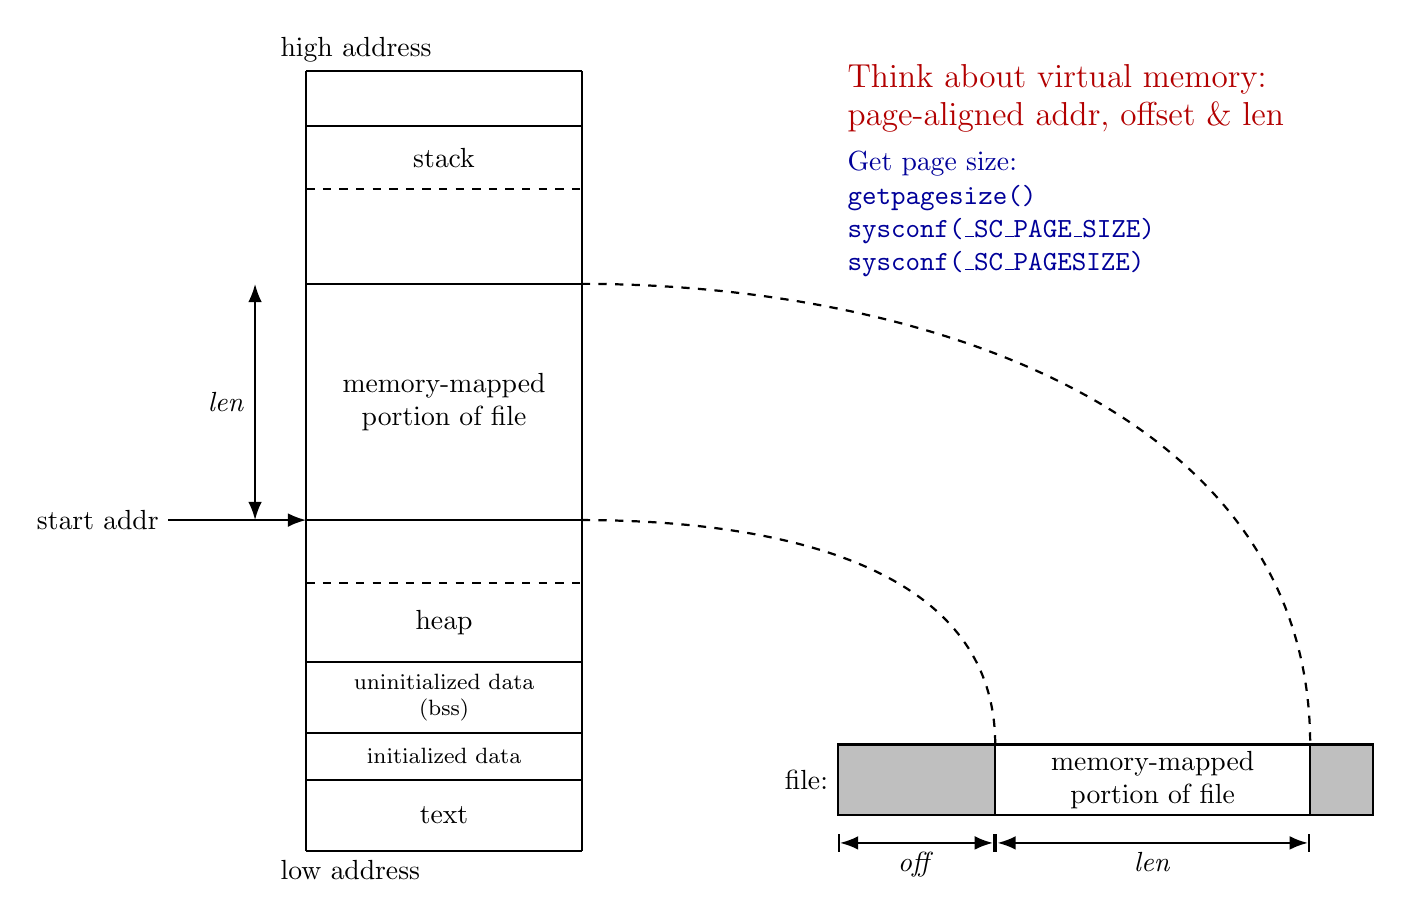
\begin{tikzpicture}[
    >=Latex,
    % 定義寬度變數,方便調整
    node distance=0cm,
]
    % --- 定義座標參數 ---
    \def\w{1.75} % 半寬 (總寬度 3.5)
    
    % Y 軸高度定義 (從上到下)
    \def\yTop{9.5}      % 頂端
    \def\yStackTop{8.8} 
    \def\yStackBot{8.0} % Stack 虛線處
    \def\yMmapTop{6.8}
    \def\yMmapBot{3.8}
    \def\yHeapTop{3.0}  % Heap 虛線處
    \def\yBssTop{2.0}
    \def\yDataTop{1.1}
    \def\yTextTop{0.5}
    \def\yBot{-0.4}     % 底端

    % --- 1. 繪製左側 Virtual Memory (整體長條) ---
    
    % 畫兩條貫穿上下的垂直線 (讓它看起來是一個整體)
    \draw[thick] (-\w, \yTop) -- (-\w, \yBot);
    \draw[thick] (\w, \yTop) -- (\w, \yBot);
    
    % 畫水平分隔線
    \draw[thick] (-\w, \yTop) -- (\w, \yTop);       % 頂部封口
    \draw[thick] (-\w, \yStackTop) -- (\w, \yStackTop); % Stack 上緣
    \draw[dashed, thick] (-\w, \yStackBot) -- (\w, \yStackBot); % Stack 下緣 (虛線)
    
    \draw[thick] (-\w, \yMmapTop) -- (\w, \yMmapTop);   % Mmap 上緣
    \draw[thick] (-\w, \yMmapBot) -- (\w, \yMmapBot);   % Mmap 下緣
    
    \draw[dashed, thick] (-\w, \yHeapTop) -- (\w, \yHeapTop); % Heap 上緣 (虛線)
    \draw[thick] (-\w, \yBssTop) -- (\w, \yBssTop);     % Heap 下緣 / BSS 上緣
    \draw[thick] (-\w, \yDataTop) -- (\w, \yDataTop);   % BSS 下緣 / Data 上緣
    \draw[thick] (-\w, \yTextTop) -- (\w, \yTextTop);   % Data 下緣 / Text 上緣
    \draw[thick] (-\w, \yBot) -- (\w, \yBot);       % 底部封口

    % --- 2. 標註文字 ---
    
    % 左側標籤
    \node[anchor=south west] at (-2.2, \yTop) {high address};
    \node[anchor=north west] at (-2.2, \yBot) {low address};

    % 區塊內容文字
    \node at (0, 8.4) {stack};
    \node[align=center] at (0, 5.3) {memory-mapped\\portion of file};
    \node at (0, 2.5) {heap};
    \node[align=center, font=\footnotesize] at (0, 1.55) {uninitialized data\\(bss)};
    \node[font=\footnotesize] at (0, 0.8) {initialized data};
    \node at (0, 0.05) {text};

    % --- 3. 尺寸標註箭頭 ---
    
    % Start Address
    \draw[->, thick] (-3.5, \yMmapBot) -- (-\w, \yMmapBot);
    \node[anchor=east] at (-3.5, \yMmapBot) {start addr};

    % Length (Vertical)
    \draw[<->, thick] (-2.4, \yMmapBot) -- (-2.4, \yMmapTop);
    \node[anchor=east] at (-2.4, 5.3) {\textit{len}};

    % --- 4. 右側 File Layout ---
    
    \def\fileY{0.5}
    \def\fileStartX{5}
    \def\fileH{0.45} % 檔案高度的一半
    
    \node[anchor=east] at (\fileStartX, \fileY) {file:};
    
    % 畫檔案 (左灰、中白、右灰)
    \draw[thick, fill=gray!50] (\fileStartX, \fileY-\fileH) rectangle (\fileStartX+2, \fileY+\fileH);
    \draw[thick] (\fileStartX+2, \fileY-\fileH) rectangle (\fileStartX+6, \fileY+\fileH); % Mapped part
    \draw[thick, fill=gray!50] (\fileStartX+6, \fileY-\fileH) rectangle (\fileStartX+6.8, \fileY+\fileH);
    
    \node[align=center] at (\fileStartX+4, \fileY) {memory-mapped\\portion of file};
    
    % 檔案尺寸標註
    \draw[|<->|, thick] (\fileStartX, \fileY-0.8) -- (\fileStartX+2, \fileY-0.8);
    \node[below] at (\fileStartX+1, \fileY-0.8) {\textit{off}};
    
    \draw[|<->|, thick] (\fileStartX+2, \fileY-0.8) -- (\fileStartX+6, \fileY-0.8);
    \node[below] at (\fileStartX+4, \fileY-0.8) {\textit{len}};

    % --- 5. 連接虛線 (Mapping Lines) ---
    
    % 從記憶體 Mmap 區塊的右上/右下 連接到 檔案對應區塊
    \draw[dashed, thick] (\w, \yMmapTop) to[out=0, in=90] (\fileStartX+6, \fileY+\fileH);
    \draw[dashed, thick] (\w, \yMmapBot) to[out=0, in=90] (\fileStartX+2, \fileY+\fileH);

    % --- 6. 右上角文字註解 ---
    
    \node[align=left, anchor=south west, text=red!70!black, font=\large] at (5, 8.6) {
        Think about virtual memory:\\
        page-aligned addr, offset \& len
    };
    
    \node[align=left, anchor=north west, text=blue!60!black, font=\normalsize] at (5, 8.6) {
        Get page size:\\
        \texttt{getpagesize()}\\
        \texttt{sysconf(\_SC\_PAGE\_SIZE)}\\
        \texttt{sysconf(\_SC\_PAGESIZE)}
    };

\end{tikzpicture}

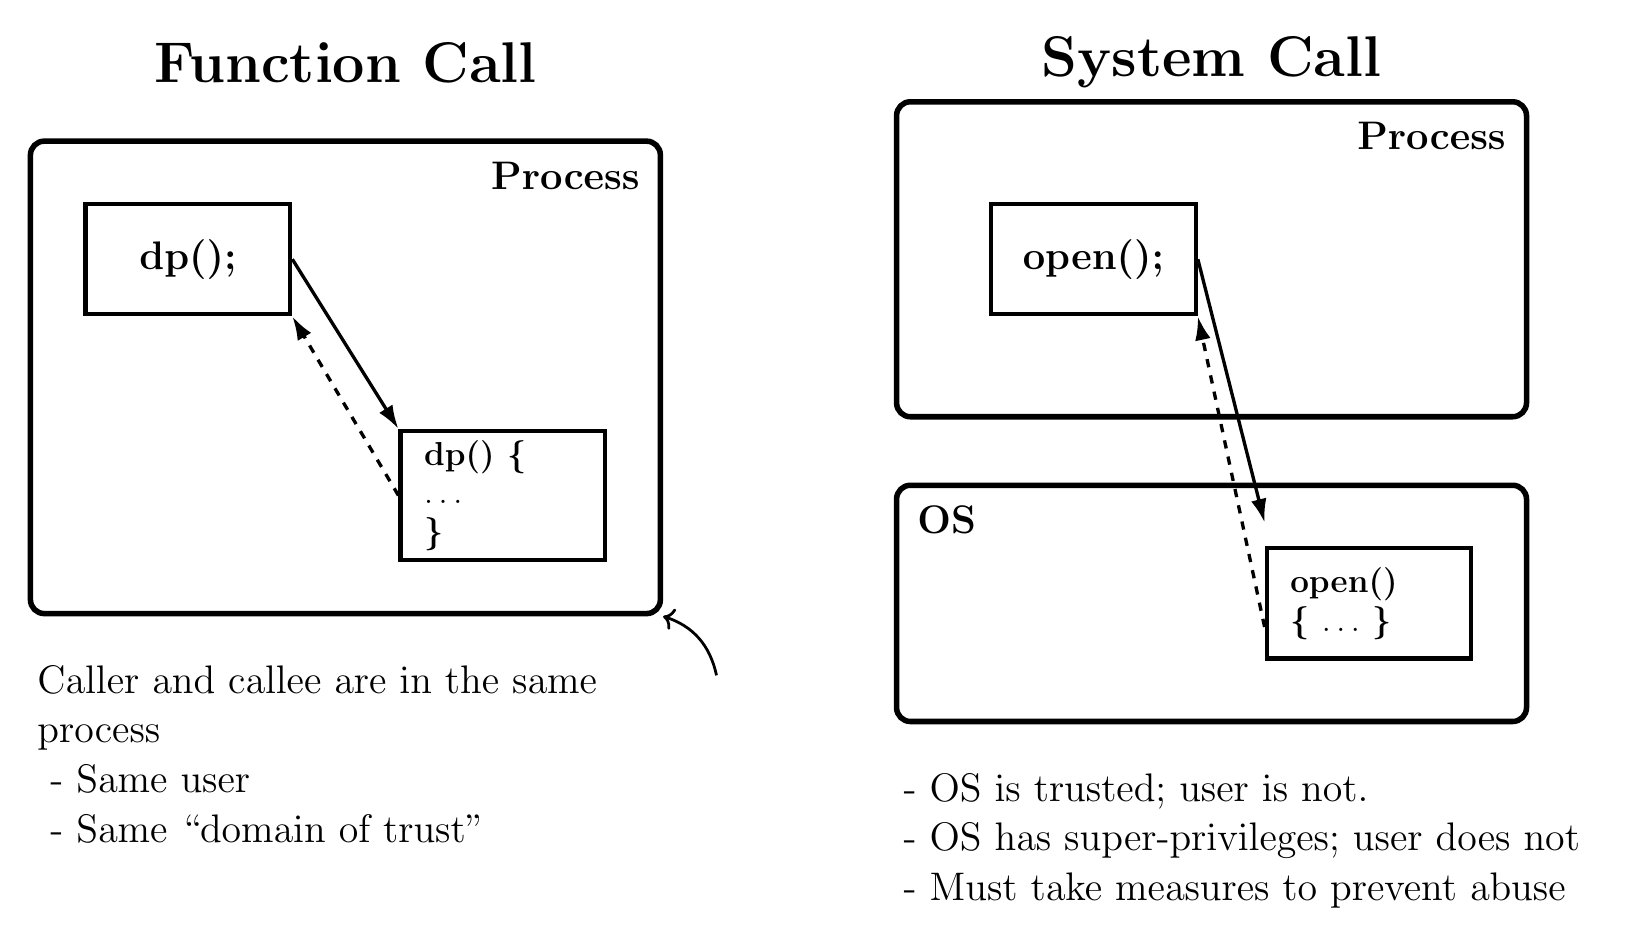
\begin{tikzpicture}[node distance=1cm and 1cm]
\node[font=\bfseries\huge] (title1) at (0, 1) {Function Call};
\node[draw=black, line width=2pt, fill=white, rounded corners=5pt, minimum width=8cm, minimum height=6cm] (proc1) at (0, -3) {};
\node[font=\bfseries\Large, anchor=north east, xshift=-5pt, yshift=-5pt, text=black] at (proc1.north east) {Process};
\node[draw=black, line width=1.5pt, fill=white, minimum width=2.6cm, minimum height=1.4cm, text=black, font=\bfseries\Large, align=center, anchor=center] (call1) at ($(proc1.center) + (-2, 1.5)$) {dp();};
\node[draw=black, line width=1.5pt, fill=white, minimum width=2.6cm, minimum height=1.4cm, text=black, font=\bfseries\large, align=left, anchor=center] (callee1) at ($(proc1.center) + (2, -1.5)$) {\begin{minipage}{2cm}dp() \{ \\ \ \ $\dots$ \\ \}\end{minipage}};
\draw[->, -{Latex[length=3mm, width=2mm]}, line width=1.2pt, draw=black] (call1.east) -- (callee1.north west);
\draw[->, -{Latex[length=3mm, width=2mm]}, line width=1.2pt, draw=black, dashed] (callee1.west) -- (call1.south east);
\node[below=0.5cm of proc1.south west, anchor=north west, align=left, font=\Large, text width=8.5cm] (text1) {Caller and callee are in the same\\ process\\ \ - Same user\\ \ - Same ``domain of trust''};
\draw[->, line width=1pt, bend right=30, draw=black] ($(text1.east) + (0, 1)$) to (proc1.south east);
\def\rightoffset{11cm}
\node[font=\bfseries\huge] (title2) at (\rightoffset, 1) {System Call};
\node[draw=black, line width=2pt, fill=white, rounded corners=5pt, minimum width=8cm, minimum height=4cm] (proc2) at (\rightoffset, -1.5) {};
\node[font=\bfseries\Large, anchor=north east, xshift=-5pt, yshift=-5pt, text=black] at (proc2.north east) {Process};
\node[draw=black, line width=1.5pt, fill=white, minimum width=2.6cm, minimum height=1.4cm, text=black, font=\bfseries\Large, align=center, anchor=center] (call2) at ($(proc2.center) + (-1.5, 0)$) {open();};
\node[draw=black, line width=2pt, fill=white, rounded corners=5pt, minimum width=8cm, minimum height=3cm, below=0.8cm of proc2] (os) {};
\node[font=\bfseries\Large, anchor=north west, xshift=5pt, yshift=-5pt, text=black] at (os.north west) {OS};
\node[draw=black, line width=1.5pt, fill=white, minimum width=2.6cm, minimum height=1.4cm, text=black, font=\bfseries\large, align=left, anchor=center] (callee2) at ($(os.center) + (2, 0)$) {\begin{minipage}{2cm}open() \\ \{ $\dots$ \}\end{minipage}};
\draw[->, -{Latex[length=3mm, width=2mm]}, line width=1.2pt, draw=black] (call2.east) -- ($(callee2.north west) + (0, 0.3)$);
\draw[->, -{Latex[length=3mm, width=2mm]}, line width=1.2pt, draw=black, dashed] ($(callee2.west) + (0, -0.3)$) -- (call2.south east);
\node[below=0.5cm of os.south west, anchor=north west, align=left, font=\Large, text width=9cm] (text2) {- OS is trusted; user is not.\\ - OS has super-privileges; user does not\\ - Must take measures to prevent abuse};
\end{tikzpicture}

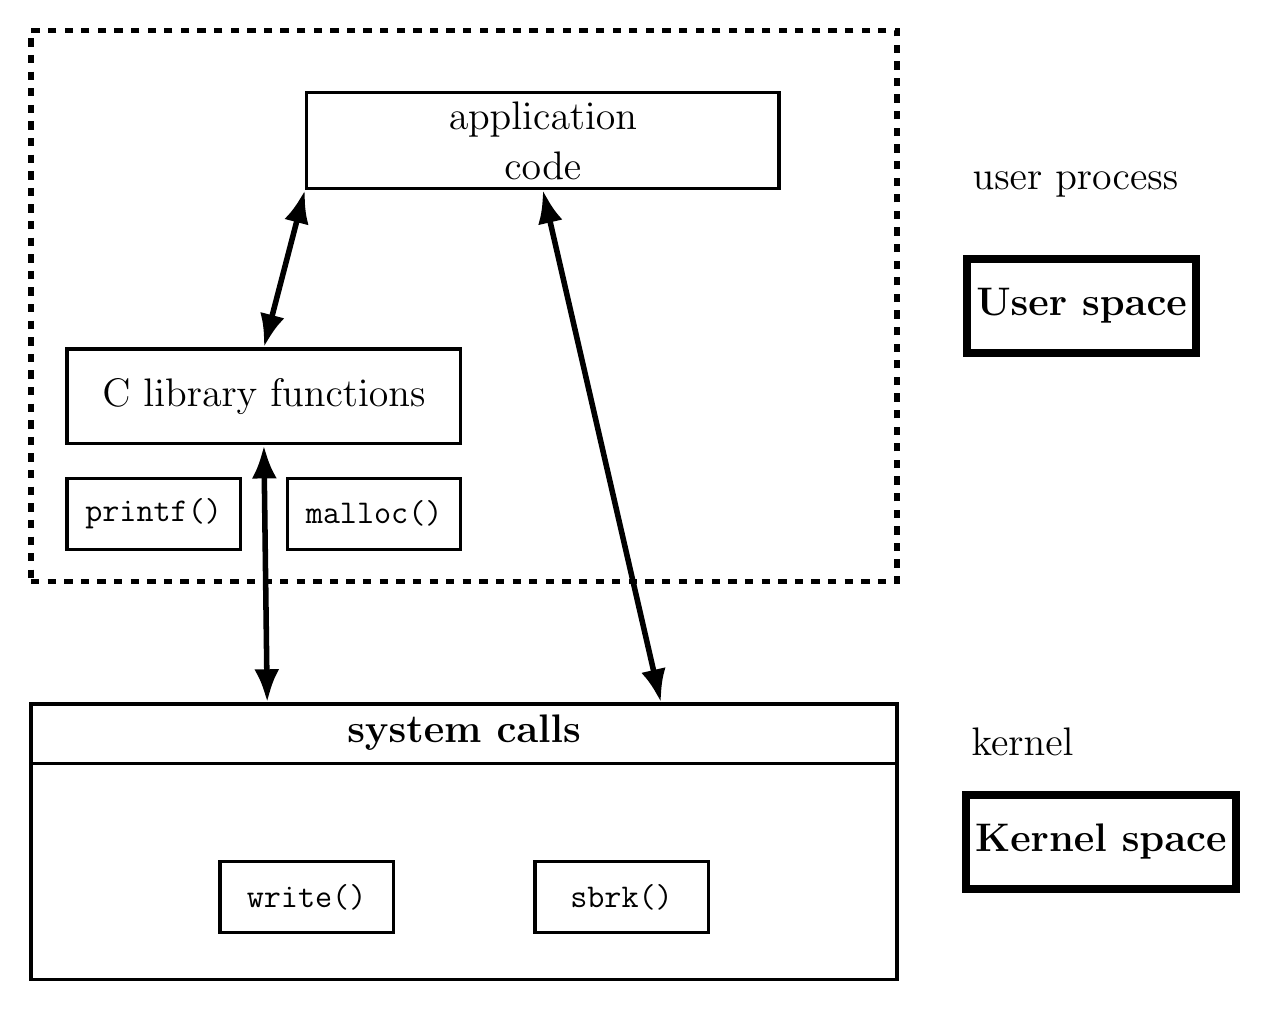
\begin{tikzpicture}[node distance=1cm]
\tikzset{basicbox/.style={draw=black, line width=1.2pt, fill=white, align=center, text=black}, smallbox/.style={basicbox, font=\large, minimum width=2.2cm, minimum height=0.9cm}, arrowstyle/.style={->, >=Latex, line width=2pt, black}}
\node[basicbox, minimum width=11cm, minimum height=3.5cm] (kernelbg) at (0,0) {};
\draw[line width=1.2pt] ($(kernelbg.north west)!(0,1cm)!(kernelbg.south west)$) -- ($(kernelbg.north east)!(0,1cm)!(kernelbg.south east)$);
\node at ($(kernelbg.north)!0.5!(kernelbg.north |- 0,1cm)$) [font=\bfseries\Large] {system calls};
\node[smallbox] (write) at ($(kernelbg.center) + (-2, -0.7)$) {\texttt{write()}};
\node[smallbox] (sbrk) at ($(kernelbg.center) + (2, -0.7)$) {\texttt{sbrk()}};
\node[draw=black, dashed, line width=2pt, minimum width=11cm, minimum height=7cm, above=1.5cm of kernelbg] (userproc) {};
\node[basicbox, minimum width=6cm, minimum height=1.2cm, font=\Large, below=0.8cm of userproc.north, xshift=1cm] (app) {application\\code};
\node[basicbox, minimum width=5cm, minimum height=1.2cm, font=\Large, below left=2cm and -2cm of app] (clib) {C library functions};
\node[smallbox, below=0.4cm of clib.south west, anchor=north west] (printf) {\texttt{printf()}};
\node[smallbox, below=0.4cm of clib.south east, anchor=north east] (malloc) {\texttt{malloc()}};
\draw[arrowstyle, <->] (app.south west) -- (clib.north);
\draw[arrowstyle, <->] (clib.south) -- ($(kernelbg.north) + (-2.5,0)$);
\draw[arrowstyle, <->] (app.south) -- ($(kernelbg.north) + (2.5,0)$);
\node[anchor=west, font=\Large] at ($(userproc.north east) + (0.8, -2.0)$) {user process};
\node[draw=black, line width=3pt, fill=white, text=black, font=\bfseries\Large, anchor=west, right=0.8cm of userproc.east, minimum height=1.2cm] {User space};
\node[anchor=west, font=\Large] at ($(kernelbg.north east) + (0.8, -0.5)$) {kernel};
\node[draw=black, line width=3pt, fill=white, text=black, font=\bfseries\Large, anchor=west, right=0.8cm of kernelbg.east, minimum height=1.2cm] {Kernel space};
\end{tikzpicture}

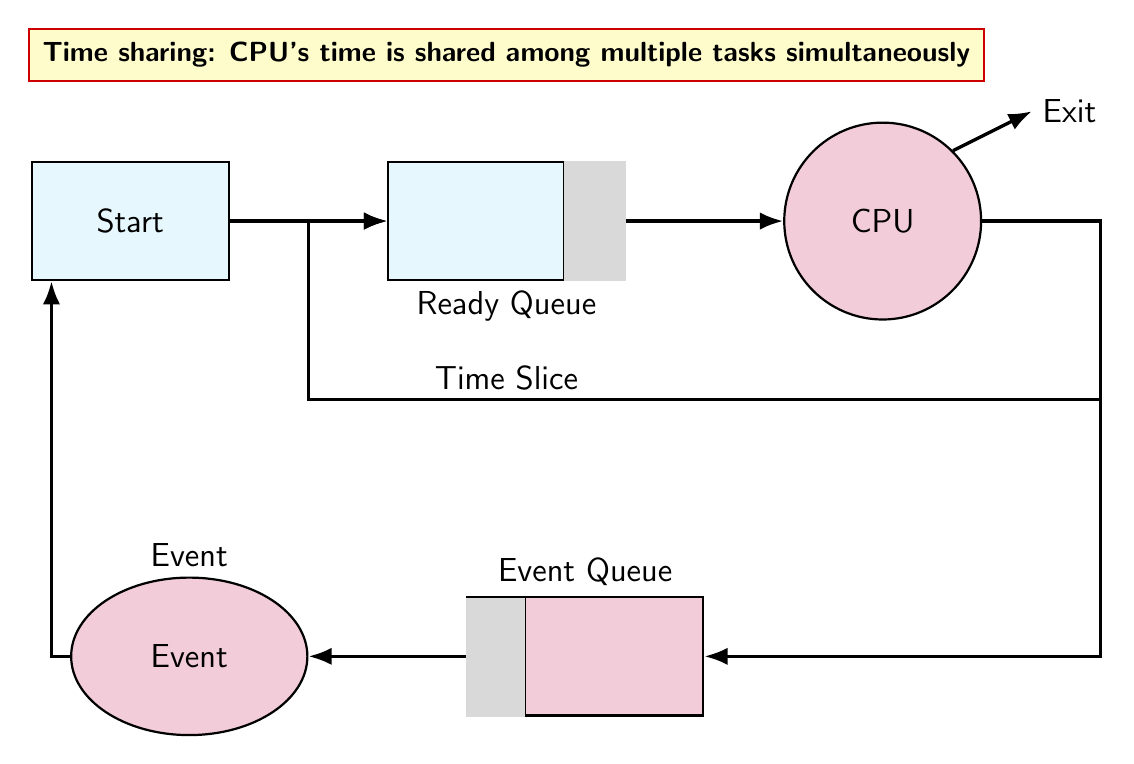
\begin{tikzpicture}[
    font=\sffamily\large,
    >=Latex,
    thick,
    % 定義通用樣式
    block/.style={draw, rectangle, minimum width=2.5cm, minimum height=1.5cm, align=center, fill=white},
    queue/.style={draw, rectangle, minimum width=3cm, minimum height=1.5cm, fill=white},
    cpu/.style={draw, circle, minimum size=2.5cm, fill=white, align=center},
    event/.style={draw, ellipse, minimum width=3cm, minimum height=2cm, fill=white, align=center},
    line/.style={draw, ->, very thick}
]

    % --- 1. Nodes (節點) ---

    % Start Node
    \node[block, fill=cyan!10] (start) {Start};

    % Ready Queue
    % 使用 label 在下方標示文字
    \node[queue, right=2cm of start, label=below:Ready Queue, fill=cyan!10] (readyq) {};
    % 畫 Ready Queue 內部的分隔線 (裝飾)
    \draw (readyq.south west) ++(2.25cm,0) -- ++(0,1.5cm);
    \draw (readyq.south west) ++(2.5cm,0) -- ++(0,1.5cm);
    \draw (readyq.south west) ++(2.75cm,0) -- ++(0,1.5cm);
    % 為了模擬圖片中的彩色區塊,這裡用灰階或淡色示意,若要純黑白可移除
    \fill[gray!30] ($(readyq.south west)+(2.25,0)$) rectangle (readyq.north east);

    % CPU
    \node[cpu, right=2cm of readyq, fill=purple!20] (cpu) {CPU};

    % Event Queue (位於下方)
    \node[queue, below=4cm of readyq, xshift=1cm, label=above:Event Queue, fill=purple!20] (eventq) {};
    % Event Queue 內部線條
    \draw (eventq.south west) ++(0.25cm,0) -- ++(0,1.5cm);
    \draw (eventq.south west) ++(0.5cm,0) -- ++(0,1.5cm);
    \draw (eventq.south west) ++(0.75cm,0) -- ++(0,1.5cm);
    \fill[gray!30] (eventq.south west) rectangle ($(eventq.south west)+(0.75,1.5)$);

    % Event Node (橢圓形)
    \node[event, left=2cm of eventq, label=above:Event, fill=purple!20] (event_node) {Event};


    % --- 2. Paths (路徑連線) ---

    % Start -> Ready Queue
    \draw[line] (start.east) -- (readyq.west);

    % Ready Queue -> CPU
    \draw[line] (readyq.east) -- (cpu.west);

    % CPU -> Exit
    \draw[line] (cpu.45) -- ++(1, 0.5) node[right] {Exit};

    % --- Feedback Loops (回授路徑) ---

    % 設定共用的右側轉折點 X 座標
    \coordinate (feedback_start) at ($(cpu.east) + (1.5, 0)$);

    % Path 1: Time Slice (CPU -> Ready Queue)
    % 路徑:CPU右 -> 下 -> 左 -> 上 -> Ready Queue左
    \draw[line] (cpu.east) -- (feedback_start) |- ($(readyq.south) - (0, 1.5)$) coordinate (mid_point) -| ($(start.east)!0.5!(readyq.west)$) -- (readyq.west);
    
    % 標示 Time Slice 文字
    \node[above] at (mid_point -| readyq.south) {Time Slice};

    % Path 2: Event Wait (CPU -> Event Queue)
    % 路徑:從 Time Slice 的線分出來 -> 進入 Event Queue 右側
    \draw[line] (feedback_start) |- (eventq.east);

    % Path 3: Event -> Ready Queue
    % 路徑:Event Queue左 -> Event圓 -> 左 -> 上 -> Ready Queue左
    \draw[line] (eventq.west) -- (event_node.east);
    \draw[line] (event_node.west) -| ($(start.south) - (1, 0)$);


    % --- 3. Top Title (頂部標題) ---
    \node[above=1cm of readyq, draw=red!80!black, fill=yellow!20, inner sep=5pt, font=\bfseries\sffamily] {Time sharing: CPU's time is shared among multiple tasks simultaneously};

\end{tikzpicture}

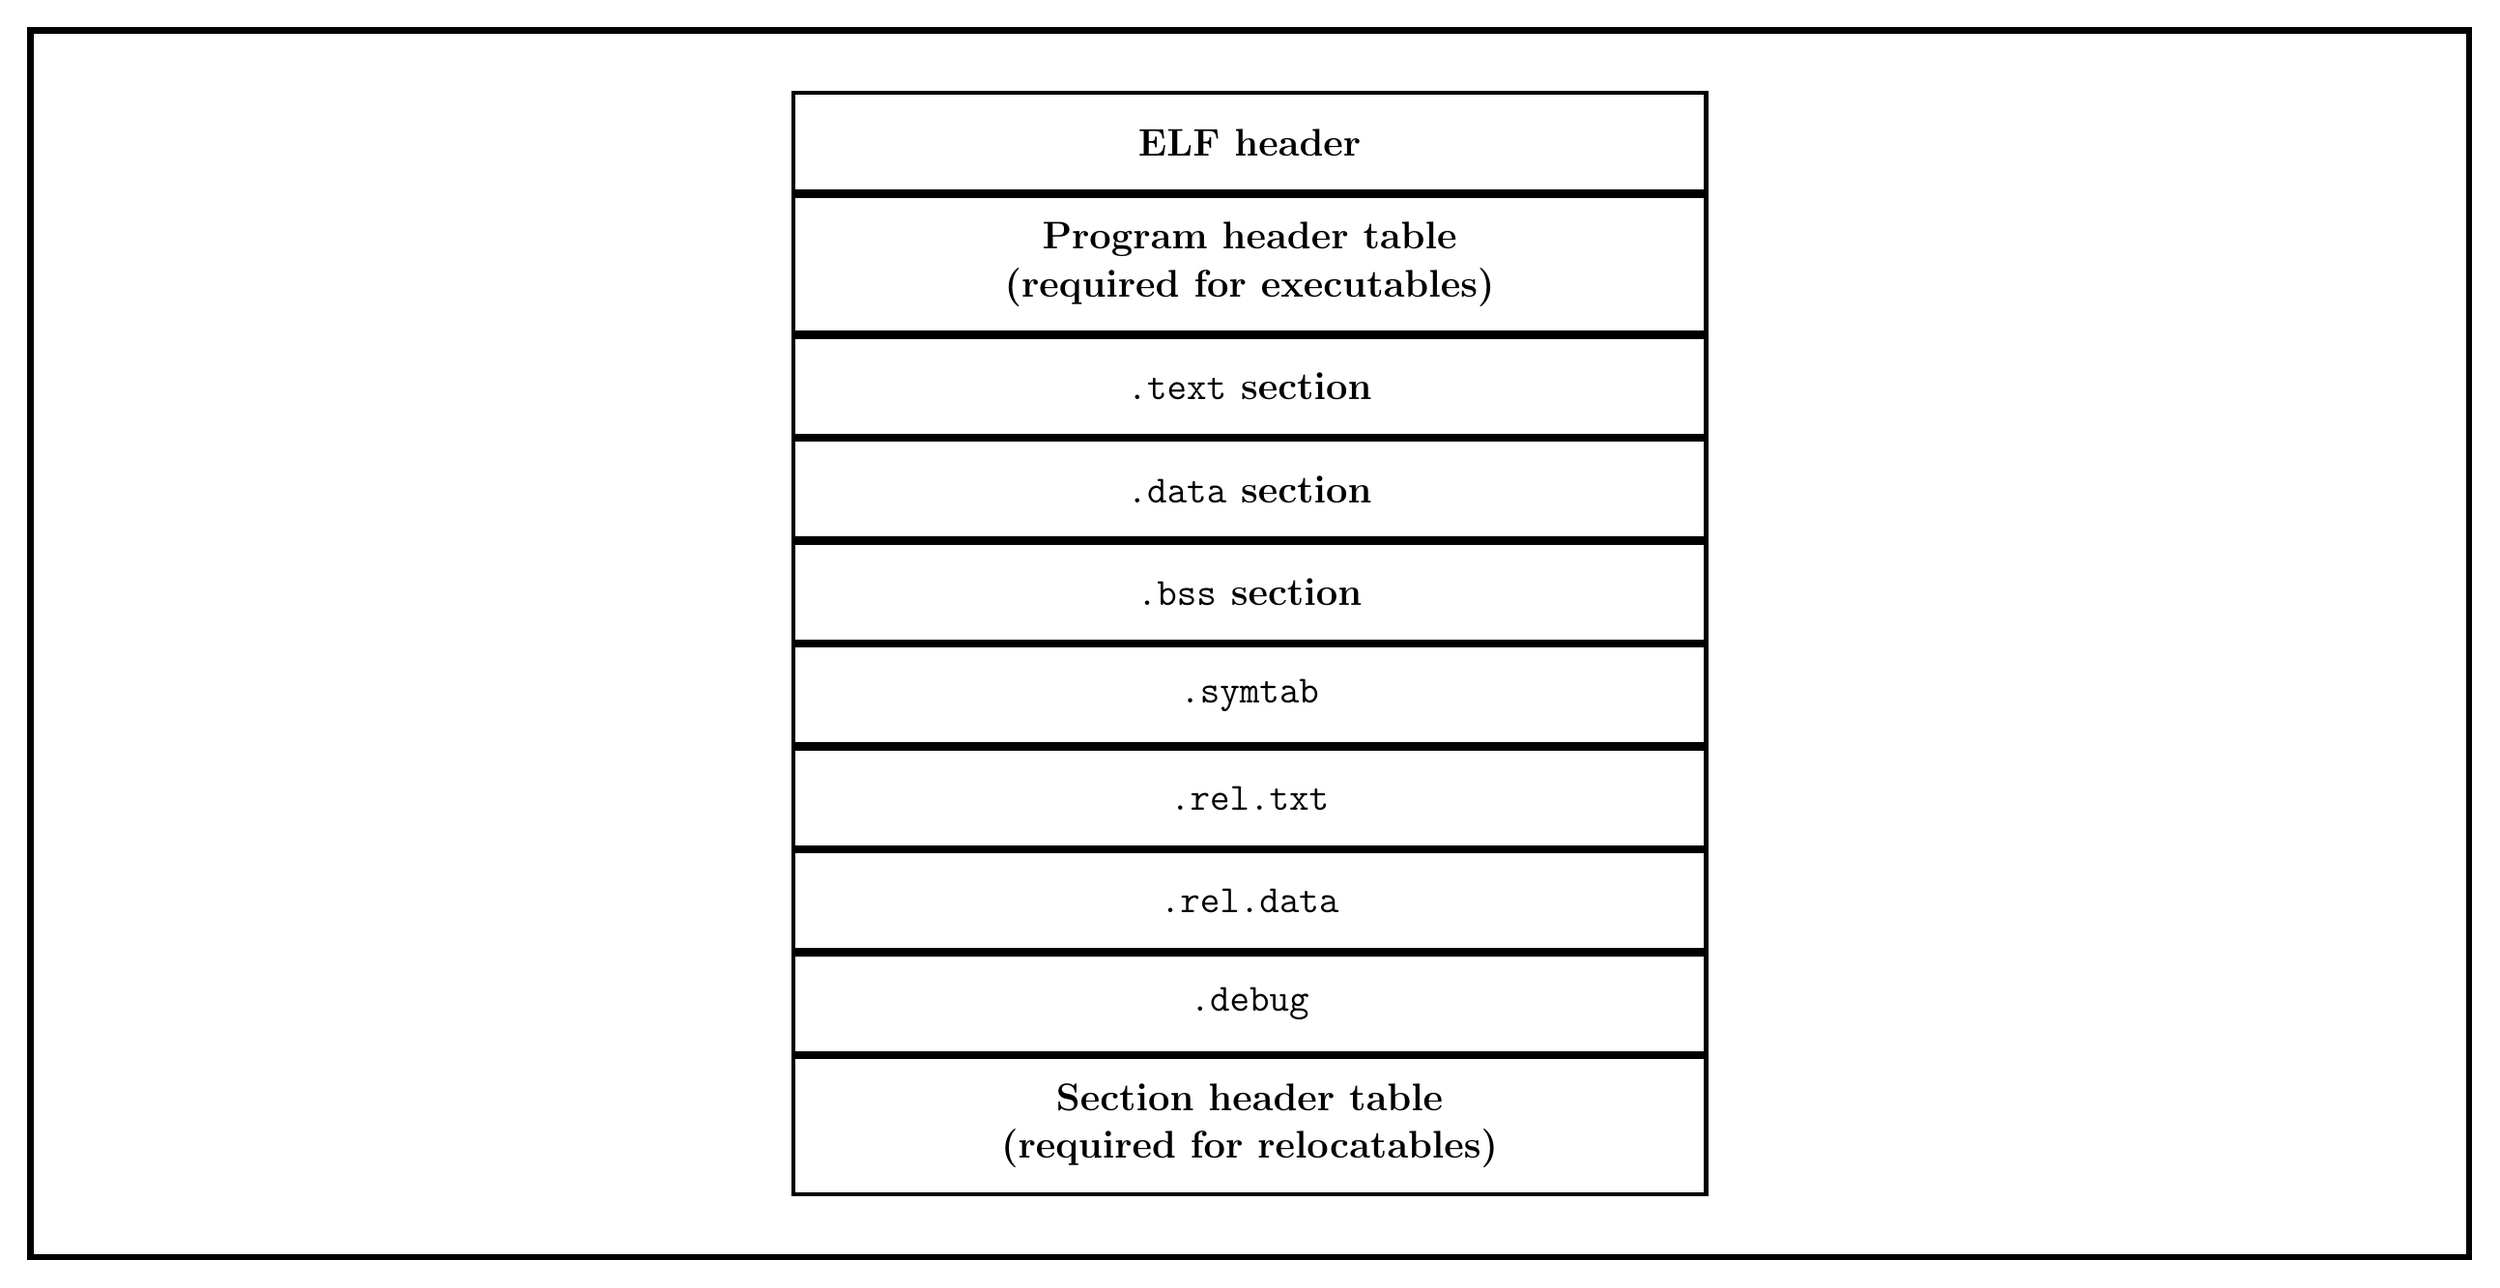
\begin{tikzpicture}

  % --- 定義樣式 ---
  \tikzset{
    % 內部表格每一列的樣式:黑框、白底、黑字、粗體
    elfbox/.style={
      draw=black,
      line width=1.5pt,
      fill=white,
      text=black,
      font=\bfseries\Large,
      align=center,
      minimum width=12cm, % 設定內部表格的固定寬度
      minimum height=1.3cm,
      anchor=north, % 對齊點設為上方中點,方便緊密堆疊
      inner sep=5pt
    },
    % 最外層大框的樣式
    outerframe/.style={
      draw=black,
      line width=2.5pt,
      inner sep=0pt % 不需要額外內部間距,由定位點決定
    }
  }

  % --- 繪製內部表格結構 ---
  % 使用 below=0pt 確保方塊之間緊密相連沒有縫隙

  % 1. ELF Header
  \node[elfbox] (header) at (0,0) {ELF header};

  % 2. Program Header Table
  \node[elfbox, below=0pt of header, minimum height=1.8cm] (pheader) {Program header table\\(required for executables)};

  % 3. Sections (.text, .data, .bss)
  \node[elfbox, below=0pt of pheader] (text) {\texttt{.text} section};
  \node[elfbox, below=0pt of text] (data) {\texttt{.data} section};
  \node[elfbox, below=0pt of data] (bss) {\texttt{.bss} section};

  % 4. Symbols and Relocations
  \node[elfbox, below=0pt of bss] (symtab) {\texttt{.symtab}};
  \node[elfbox, below=0pt of symtab] (reltxt) {\texttt{.rel.txt}};
  \node[elfbox, below=0pt of reltxt] (reldata) {\texttt{.rel.data}};

  % 5. Debug
  \node[elfbox, below=0pt of reldata] (debug) {\texttt{.debug}};

  % 6. Section Header Table (底部)
  \node[elfbox, below=0pt of debug, minimum height=1.8cm] (sheader) {Section header table\\(required for relocatables)};


  % --- 繪製最外層的扁長方形外框 ---

  % 定義左右留白的寬度 (例如:兩側各留 4cm)
  \def\hpadding{10cm}
  % 定義上下留白的高度 (稍微留一點點即可)
  \def\vpadding{0.8cm}

  % 計算外框的左上角和右下角座標
  % 左上角:以最上面的 header 的左上角為基準,向左和向上偏移
  \coordinate (outerTL) at ($(header.north west) + (-\hpadding, \vpadding)$);
  % 右下角:以最下面的 sheader 的右下角為基準,向右和向下偏移
  \coordinate (outerBR) at ($(sheader.south east) + (\hpadding, -\vpadding)$);

r  \node[outerframe, fit=(outerTL) (outerBR)] {};

\end{tikzpicture}

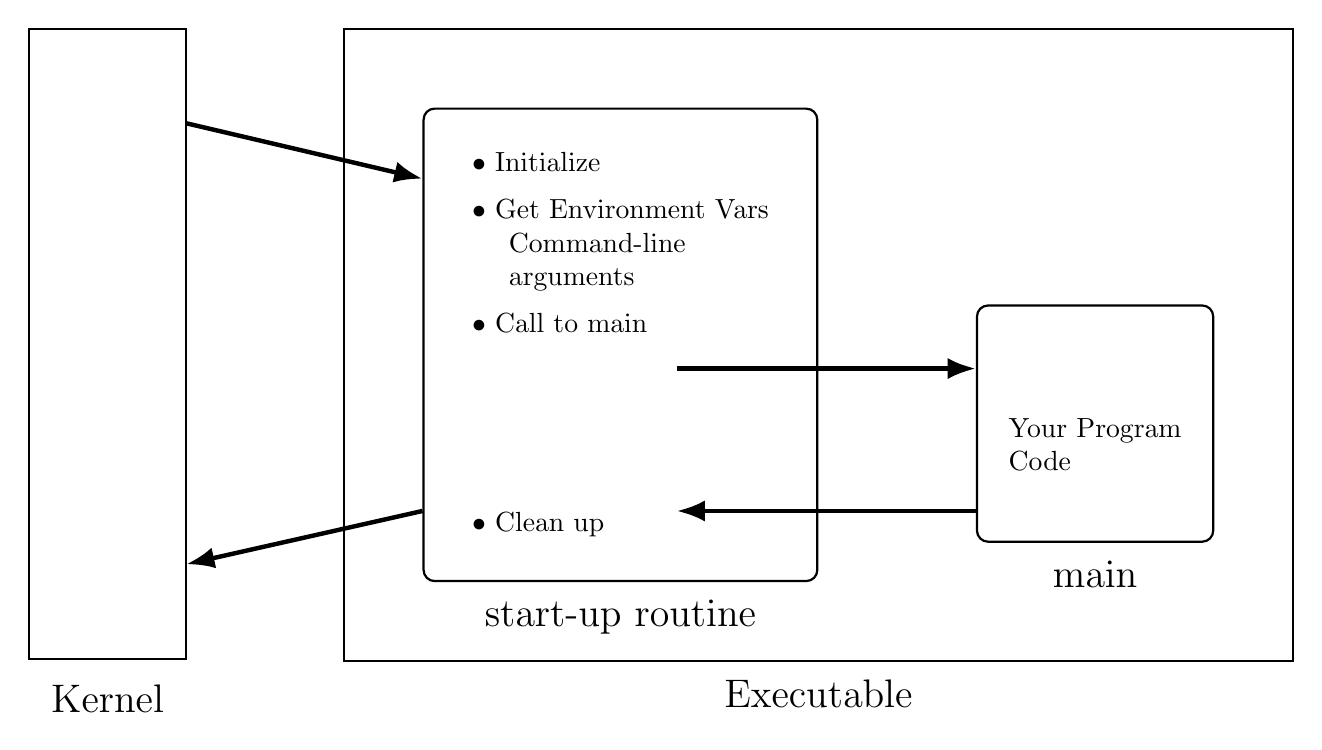
\begin{tikzpicture}[
    >=Latex, % 使用標準箭頭樣式
    node distance=2cm,
    thick, % 線條加粗
    % 定義樣式
    block/.style={
        draw, 
        rounded corners, 
        fill=white, 
        align=left,
        inner sep=10pt
    },
    kernel/.style={
        draw, 
        fill=white, 
        minimum height=8cm, 
        minimum width=2cm,
        outer sep=0pt
    },
    mainblock/.style={
        draw,
        rounded corners,
        fill=white,
        minimum size=3cm,
        align=left
    }
]

    % --- 1. Kernel (Left) ---
    \node[kernel] (kernel) {};
    \node[below=0.2cm] at (kernel.south) {\Large Kernel};

    % --- 2. Start-up Routine (Center) ---
    % 我們手動調整文字內容與行距
    \node[block, right=3cm of kernel.north east, yshift=-1cm, anchor=north west, minimum height=6cm, minimum width=5cm] (startup) {
        $\bullet$ Initialize\\[0.5em]
        $\bullet$ Get Environment Vars\\
        \hspace{1em} Command-line\\
        \hspace{1em} arguments\\[0.5em]
        $\bullet$ Call to main\\[6em] % 留空給箭頭回流
        $\bullet$ Clean up
    };
    \node[below=0.1cm] at (startup.south) {\Large start-up routine};

    % --- 3. Main Function (Right) ---
    % 定位在 startup 的右側,垂直位置稍微對齊中間偏下
    \node[mainblock, right=2cm of startup, yshift=-1cm] (main) {
        \\[1em] % 稍微往下推一點
        Your Program\\
        Code
    };
    \node[below=0.1cm] at (main.south) {\Large main};

    % --- 4. Executable Container (Big Box) ---
    % 畫一個大框包住 Start-up 和 Main
    \node[draw, inner sep=1cm, fit=(startup) (main) (main.south |- startup.south)] (execbox) {};
    \node[below=0.1cm] at (execbox.south) {\Large Executable};

    % --- 5. Arrows (連線) ---
    
    % Arrow 1: Kernel -> Initialize
    % 透過計算座標來對齊文字
    \draw[->, ultra thick] ($(kernel.north east)!0.15!(kernel.south east)$) -- ($(startup.north west)!0.15!(startup.south west)$);

    % Arrow 2: Call to main -> Main block
    % 從 startup 中間偏上的位置指出去
    \draw[->, ultra thick] ($(startup.north east)!0.55!(startup.south east) + (-1.8, 0)$) -- (main.west |- {$(startup.north east)!0.55!(startup.south east)$});

    % Arrow 3: Main block -> Clean up (Backwards)
    % 從 main 下方指回 startup 下方
    \draw[->, ultra thick] ($(main.west |- {$(startup.north east)!0.85!(startup.south east)$})$) -- ($(startup.north east)!0.85!(startup.south east) + (-1.8, 0)$);

    % Arrow 4: Clean up -> Kernel
    \draw[->, ultra thick] ($(startup.north west)!0.85!(startup.south west)$) -- ($(kernel.north east)!0.85!(kernel.south east)$);

\end{tikzpicture}

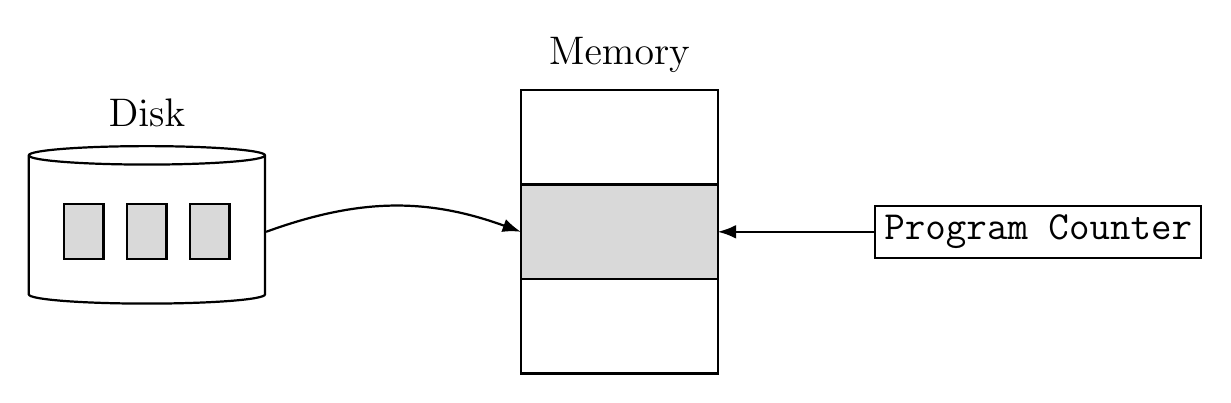
\begin{tikzpicture}[
    font=\Large, % 設定字體為無襯線且較大
    thick, % 線條加粗
    >=Latex, % 設定箭頭樣式
    % 定義通用樣式
    box/.style={
        draw, 
        fill=white, 
        minimum width=2.5cm, 
        outer sep=0pt % 讓方塊邊框緊貼
    },
    inner block/.style={
        draw, 
        fill=white, 
        minimum width=0.5cm, 
        minimum height=0.7cm,
        fill=gray!30
    }
]
    % --- 1. Disk (Left) ---
    % 使用 cylinder 形狀來畫圓柱體
    \node[
        cylinder, 
        shape border rotate=90, % 旋轉使圓柱直立
        draw, 
        fill=white, 
        minimum height=2cm, 
        minimum width=3cm
    ] (disk) {};
    
    % Disk 內部的檔案區塊 (模擬原圖的小方塊)
    % 使用相對座標定位
    \node[inner block] at ($(disk.center) + (-0.8, 0)$) {};
    \node[inner block] at ($(disk.center) + (0.0, 0)$) {};
    \node[inner block] at ($(disk.center) + (0.8, 0)$) {};
    
    % Disk 標籤
    \node[above=0.1cm of disk.top] {Disk};

    % --- 2. Memory (Center) ---
    % 分為上、中、下三塊
    % 頂部區塊
    \node[box, minimum height=1.2cm, right=6cm of disk.center, anchor=center, yshift=1.2cm] (mem_top) {};
    % 中間區塊 (被指向的目標)
    \node[box, minimum height=1.2cm, below=0pt of mem_top, fill=gray!30] (mem_mid) {};
    % 底部區塊
    \node[box, minimum height=1.2cm, below=0pt of mem_mid] (mem_bot) {};
    
    % Memory 標籤
    \node[above=0.1cm of mem_top] {Memory};

    % --- 3. Program Counter (Right) ---
    \node[right=2cm of mem_mid, box] (pc) {\texttt{Program Counter}};

    % --- 4. Arrows (連線) ---
    
    % Arrow: Disk -> Memory (帶有彎曲)
    \draw[->, thick] (disk.east) to[bend left=20] (mem_mid.west);

    % Arrow: Program Counter -> Memory (直線)
    \draw[->, thick] (pc.west) -- (mem_mid.east);

\end{tikzpicture}

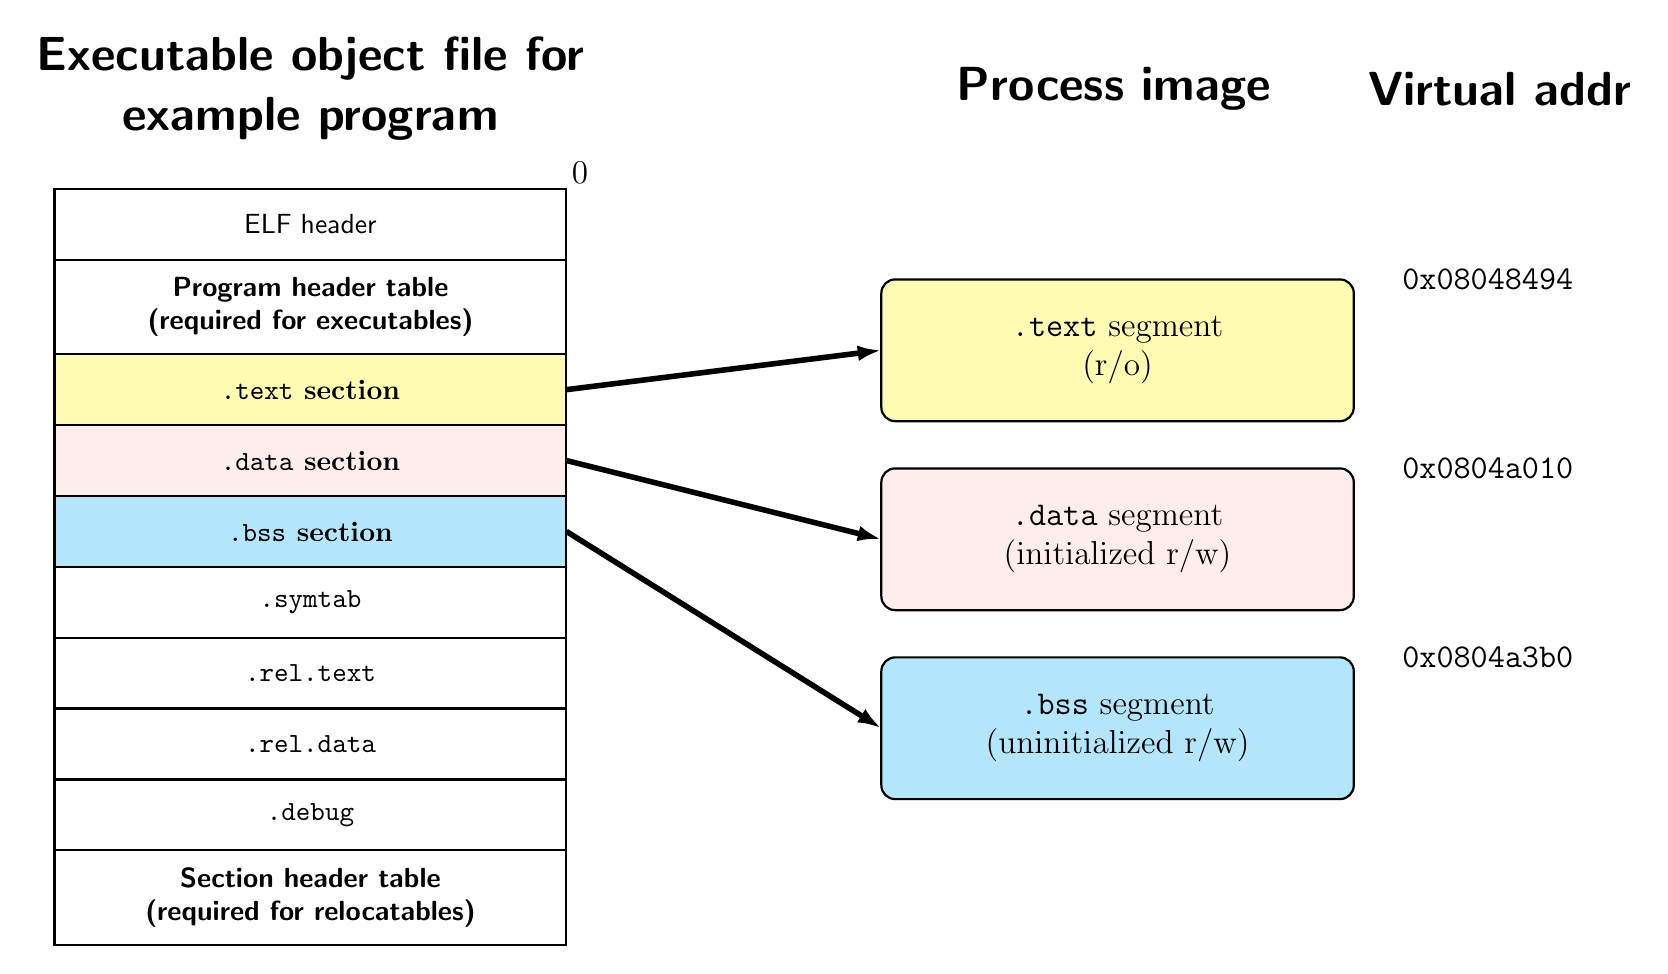
\begin{tikzpicture}[
    font=\sffamily, % 使用無襯線字體
    thick, % 線條加粗
    >={Latex[length=3mm, width=2mm]}, % 設定箭頭樣式
    node distance=0cm, % 節點間緊密排列
    outer sep=0pt, % 無外部間距
    % --- 樣式定義 ---
    % 基本黑框白底方塊
    basic box/.style={
        draw=black,
        fill=white,
        minimum width=6.5cm,
        minimum height=0.9cm,
        align=center,
        inner sep=5pt
    },
    % 標題方塊(加粗)
    header box/.style={
        basic box,
        font=\sffamily\bfseries,
        minimum height=1.2cm
    },
    % --- 彩色填充樣式 (顏色可隨意替換) ---
    text fill/.style={fill=yellow!30},
    data fill/.style={fill=pink!30},
    bss fill/.style={fill=cyan!30},
    % 左側彩色區塊樣式
    text box/.style={basic box, text fill, font=\bfseries},
    data box/.style={basic box, data fill, font=\bfseries},
    bss box/.style={basic box, bss fill, font=\bfseries},
    % 右側 Process image 區塊樣式
    segment box/.style={
        draw=black,
        minimum width=6cm,
        minimum height=1.8cm,
        align=center,
        rounded corners=5pt, % 圓角
        font=\large
    },
    % 地址標籤樣式
    addr label/.style={
        right=0.5cm,
        font=\large
    }
]

    % ====== 左側:Executable object file ======
    
    % 總標題
    \node[font=\sffamily\bfseries\LARGE, align=center] (left title) {Executable object file for\\example program};

    % 堆疊區塊
    \node[basic box, below=0.5cm of left title] (elf) {ELF header};
    % 右上角的 "0"
    \node[above right=0cm and 0cm of elf.north east, font=\large, inner sep=2pt] {0};
    
    \node[header box, below=of elf] (pht) {Program header table\\(required for executables)};
    
    % 彩色區塊
    \node[text box, below=of pht] (text sec) {\texttt{.text} section};
    \node[data box, below=of text sec] (data sec) {\texttt{.data} section};
    \node[bss box, below=of data sec] (bss sec) {\texttt{.bss} section};
    
    % 其他白色區塊
    \node[basic box, below=of bss sec] (symtab) {\texttt{.symtab}};
    \node[basic box, below=of symtab] (reltext) {\texttt{.rel.text}};
    \node[basic box, below=of reltext] (reldata) {\texttt{.rel.data}};
    \node[basic box, below=of reldata] (debug) {\texttt{.debug}};
    \node[header box, below=of debug] (sht) {Section header table\\(required for relocatables)};
    
    % 繪製左側的大外框


    % ====== 右側:Process image ======
    
    % 標題
    \node[font=\sffamily\bfseries\LARGE, right=4.5cm of left title] (right title) {Process image};
    \node[font=\sffamily\bfseries\LARGE, right=1cm of right title] (addr title) {Virtual addr};

    % 彩色 Segment 區塊與地址
    % .text segment
    \node[segment box, text fill, right=4cm of text sec, yshift=0.5cm] (text seg) {\texttt{.text} segment\\(r/o)};
    \node[addr label, yshift=0.9cm] at (text seg.east) {\texttt{0x08048494}};

    % .data segment
    \node[segment box, data fill, right=4cm of data sec, yshift=-1cm] (data seg) {\texttt{.data} segment\\(initialized r/w)};
    \node[addr label, yshift=0.9cm] at (data seg.east) {\texttt{0x0804a010}};

    % .bss segment
    \node[segment box, bss fill, right=4cm of bss sec, yshift=-2.5cm] (bss seg) {\texttt{.bss} segment\\(uninitialized r/w)};
    \node[addr label, yshift=0.9cm] at (bss seg.east) {\texttt{0x0804a3b0}};

    % ====== 箭頭連接 ======
    \draw[->, line width=2pt] (text sec.east) -- (text seg.west);
    \draw[->, line width=2pt] (data sec.east) -- (data seg.west);
    \draw[->, line width=2pt] (bss sec.east) -- (bss seg.west);

\end{tikzpicture}

\end{document}
